\chapter{Contribuição}
\label{cap_contribuicao}

Nesta secção, será relatado o trabalho realizado no intuito da componente prática do projeto e os resultados. 
% Neste caso, relevante à criação de um \textit{toolkit} e ferramentas para a extração do conteúdo de documentos antigos, em particular jornais, com melhores resultados do que os oferecidos pelas ferramentas de \acrshort{ocr} base e, possibilitando a obtenção da lógica e organização original dos mesmos.

\section{Introdução}
% Ao longo do período de inicialização da dissertação: desde a definição dos objetivos do projeto, aprofundamento da temática e estudo do estado da arte; de forma a simultaneamente acostumar com as tecnologias, assim como ganhar um melhor entendimento sobre os algoritmos a implementar e os desafios apresentados, algum trabalho prático já foi realizado. 
% Este envolve principalmente a criação de uma ferramenta para facilitar a visualização dos resultados de reconhecimento, assim como o debugging destes e alguns algoritmos preliminares para manipulação destes resultados de \acrshort{ocr}.

A discussão sobre o trabalho realizado será estruturada em 3 componentes principais.
\begin{itemize}
	\item Ferramentas do \textit{toolkit} desenvolvidas \ref{contribution_toolkit}
	\item Pipeline de aplicação do toolkit \ref{contribution_toolkit_pipeline}
% 	\item GUI de aplicação geral do \textit{toolkit}
	\item GUI editor OCR \ref{contribution_ocr_editor}
\end{itemize}

Para cada uma das secções delimitadas, será dada uma explicação do seu propósito e produto sumariado, procedido por uma discussão mais detalhada dos elementos que a constituem.

De forma geral, o código desenvolvido foi maioritariamente escrito em Python, com algumas instâncias de C.

\section{Ferramentas do \textit{toolkit} desenvolvidas}
\label{contribution_toolkit}

\subsection{Introdução}

A componente do \textit{toolkit} foi a premissa base do tema da dissertação. Um conjunto de ferramentas focado na melhoria dos resultados obtidos da aplicação de \acrshort{ocr} em documentos antigos, com especial interesse em jornais. 

Estas ferramentas são então pertinentes para os diversos passos do processo convencional de \acrshort{ocr}, i.e. pré-processamento, OCR e pós-processamento; atendendo tanto a processamento de imagem, processamento de resultados de OCR e texto, e validação de resultados.

Além dos métodos principais criados para a resolução de problemas identificados, é importante realçar certos pontos essenciais que serviram como base para o resto do trabalho. Estes são as estruturas de dados utilizadas para o tratamento dos resultados de OCR.

\subsection{Sumário}

\begin{itemize}\setlength\itemsep{-0.3em}
	\item Estruturas de dados \ref{data_structures}
	\begin{itemize}\setlength\itemsep{-0.3em}
		\item OCR Tree \ref{ocr_tree}
		\item Box \ref{box_data_structure}
	\end{itemize}
	\item Métodos \ref{contribution_methods}
	
	\begin{itemize}\setlength\itemsep{-0.3em}
		\item Processamento de resultados OCR \ref{contribution_ocr_posprocessing}
		
		\begin{itemize}\setlength\itemsep{-0.3em}
			\item Conversão de resultados OCR \ref{ocr_results_conversion}
			\item Debugging \ref{contribution_debugging}
			\item Análise de texto \ref{contribution_text_analyses}
			\item Limpeza de OCR Tree \ref{contribution_clean_ocr}
			\item Categorização de Blocos \ref{contribution_categorize_blocks}
			\item Divisão de blocos \ref{contribution_divide_blocks}
			\item Cálculo de ordem de leitura \ref{contribution_reading_order}
			\item Segmentação de resultados \ref{contribution_result_segmentation}
		\end{itemize}
		
		\item Processamento de imagem \ref{contribution_image_processing}
		\begin{itemize}\setlength\itemsep{-0.3em}
			\item Correção de ângulos de rotação
			\item Corte de sombra nas margens
			\item Binarização de imagem
			\item Identificação de delimitadores
			\item Identificação de imagens no documento
			\item Segmentação de documento
		\end{itemize}
		
		\item Processamento de texto \ref{contribution_text_processing}
		\begin{itemize}\setlength\itemsep{-0.3em}
			\item Limpeza de hifenização
			\item Geração de output
		\end{itemize}
		
		
	\end{itemize}
\end{itemize}


\subsection{Estruturas de dados}
\label{data_structures}


\subsubsection{OCR Tree}
\label{ocr_tree}

Como o produto final do projeto intende aceitar diferentes tipos de resultados OCR, i.e. resultantes de diferentes motores OCR ou de ficheiros como hOCR que já possuem os resultados, existe uma necessidade de converter estes diferentes formatos num único tipo que mantenha a informação base pretendida.

Estruturas de dados standard como \citep{hocr_doc} ou \citep{alto_doc} apresentam um resultado final semelhante e com capacidade base de armazenamento de meta-dados superior porém, sendo baseados em XML, tornam a sua manipulação mais complexa e, em múltiplos casos a informação proporcionada é além do necessário ou gera conclusões erradas quando gerado de output automático (ex.: atribuição de classes caption a blocos que são títulos). Assim sendo, embora tenha sido desenvolvido um conversor de, e para HOCR, para o atual projeto, optou-se pela criação de uma estrutura de dados própria.

Deste modo, tomando como inspiração os atributos dos resultados do Tesseract no modo de dicionário \citep{tesseract_doc}, foi implementada uma estrutura de dados no formato de árvore de dados.

A escolha de uma estrutura de árvore permite a hierarquização de blocos de acordo com o seu nível, quer exista uma divisão de nível à partida, como é o caso do Tesseract que segue: página $\longrightarrow$ bloco $\longrightarrow$ parágrafo $\longrightarrow$ linha $\longrightarrow$ palavra; ou apenas um único nível, semelhante ao Keras-OCR.

Todos os algoritmos desenvolvidos, inclusive os métodos para visualização (métodos de debugging e GUI desenvolvido), assumem e trabalham com os dados de OCR no formato desta estrutura de dados.

As características mais relevantes desta estrutura são:

\begin{itemize}\setlength\itemsep{-0.3em}
	\item \textbf{Level} : Nível/altura do nodo.
	\begin{itemize}\setlength\itemsep{-0.3em}
		\item documento : 0
		\item página 	: 1
		\item bloco		: 2
		\item parágrafo : 3
		\item linha 	: 4
		\item palavra	: 5
	\end{itemize}\setlength\itemsep{-0.3em}
	\item \textbf{(page|block|par|line|word)\_num}: Identificação da ordem (dentro de outras caixas(ex.: linha), se aplicável)
	\item \textbf{text} : Texto do bloco, normalmente apenas preenchido ao nível da palavra
	\item \textbf{conf} : Confiança no texto
	\item \textbf{id}
	\item \textbf{type} : Tipo do bloco, ex.: delimitador, título
	\item \textbf{children}
	\item \textbf{box}: Bounding box do nodo, representado pela estrutura de dados Box, que também possui métodos para transformações e verificações geométricas ou de características.
	\item Características de texto: ex.: texto iniciado (start\_text); texto não terminado (end\_text).
\end{itemize}

%% TODO : Ilustracao de uso de arvore OCR para demonstrar diferentes niveis de um documento

Construtores da classe são capazes de admitir outros atributos não base de modo a expandir a utilidade da estrutura. Construtores disponíveis: iniciação por argumentos, dicionário, ficheiro JSON e ficheiro HOCR.

Da mesma forma, conversores para estes ficheiros compreendidos para iniciação também foram desenvolvidos.

A classe possuí por métodos de transformação e análise sobre a árvore OCR que facilitam a manipulação dos resultados OCR. 

Segue-se uma lista dos métodos mais relevantes disponíveis da classe.

\highlight{id\_boxes}
 
 
\textbf{Descrição:} Adiciona identificador aos blocos.
	
\textbf{Argumentos:}
	\begin{itemize}\setlength\itemsep{-0.3em}
		\item level : lista de níveis onde adicionar identificador
		\item ids (opt): dicionário de ids a utilizar caso não se queira iniciar no 0.
		\item delimiters (opt): flag para identificar delimitadores
		\item area (opt): argumento do tipo Box, que restringe os nodos a identificar a uma dada área
		\item override (opt): flag para reescrever id se já existe.
	\end{itemize}
				
\highlight{calculate\_mean\_height}

\textbf{Descrição:} Calcula a altura média das caixas de um dado nível.
	
\textbf{Argumentos:}
\begin{itemize}\setlength\itemsep{-0.3em}
	\item level : nível a calcular
	\item conf (opt): valor de confiança de texto no caso de apenas serem relevantes caixas com certa confiança (aplicável apenas para nível de texto)
\end{itemize}

	
\highlight{is\_text\_size}

\textbf{Descrição:} Verifica se um nodo se encontra dentro do tamanho de texto.
	
\textbf{Argumentos:}
\begin{itemize}\setlength\itemsep{-0.3em}
	\item text\_size : tamanho de texto a comparar
	\item mean\_height (opt): altura do bloco, caso já tenha sido calculado
	\item range : margem de erro aceitável (relativo)
	\item level : nível das caixas usado caso seja necessário calcular a altura média
	\item conf : confiança do texto a utilizar para calcular a altura média
\end{itemize}

\highlight{is\_empty}

\textbf{Descrição:} Verifica se um nodo é vazio.
	
\textbf{Argumentos:}
\begin{itemize}\setlength\itemsep{-0.3em}
	\item conf : confiança de texto a utilizar para considerar palavras válidas
	\item only\_text : flag que dita se o tipo do bloco influencia o resultado, i.e. blocos de tipo "image" não são vazios
\end{itemize}

	
\highlight{text\_is\_title}

\textbf{Descrição:} Verifica se um nodo é potencial título.
	
\textbf{Algoritmo:} Caixa não é texto vertical e é maior do que o tamanho normal de texto.


\textbf{Argumentos:}
\begin{itemize}\setlength\itemsep{-0.3em}
	\item normal\_text\_size : tamanho de texto considerado como normal
	\item conf : confiança de texto a utilizar para considerar palavras válidas
	\item range : margem de acerto aceitável (relativo)
	\item level : nível usado para calcular o tamanho médio do bloco
\end{itemize}

	
\highlight{is\_delimiter}

\textbf{Descrição:} Verifica se um nodo é potencial delimitador.
	
\textbf{Algoritmo:} Caixa já é do tipo delimitador, ou é vazia e segue a regra:

$ box.width >= box.height*4 || box.height >= box.widht*4 $.


\textbf{Argumentos:}
\begin{itemize}\setlength\itemsep{-0.3em}
	\item conf : confiança de texto a utilizar para considerar palavras válidas
	\item only\_type : flag que dita se usa apenas o tipo do nodo para a verificação
\end{itemize}

	
\highlight{is\_image}

\textbf{Descrição:} Verifica se um nodo é potencial imagem.
	
\textbf{Algoritmo:} Caixa já é do tipo imagem ou, é vazia, não é um delimitador e é 3 vezes mais alta do que o tamanho de texto.


\textbf{Argumentos:}
\begin{itemize}\setlength\itemsep{-0.3em}
	\item conf : confiança de texto a utilizar para considerar palavras válidas
	\item text\_size : tamanho de texto a utilizar para comparação com altura da caixa
	\item only\_type : flag que dita se usa apenas o tipo do nodo para a verificação
\end{itemize}


\highlight{get\_boxes\_in\_area}

\textbf{Descrição:} Obtém todas as caixas numa dada área.


\textbf{Argumentos:}
\begin{itemize}\setlength\itemsep{-0.3em}
	\item area : área de interesse
	\item level : nível dos nodos a ir buscas. Se nível == -1, obtém todos os nodos
	\item conf : confiança de texto a utilizar para considerar nodos válidos
	\item ignore\_type : tipos de nodo a ignorar
\end{itemize}
	
	
\highlight{is\_vertical\_text}

\textbf{Descrição:} Verifica se um nodo é texto vertical.

\textbf{Argumentos:}
\begin{itemize}\setlength\itemsep{-0.3em}
	\item conf : confiança de texto a utilizar para considerar palavras válidas
\end{itemize}
	
\textbf{Algoritmo:}

\begin{breakablealgorithm}
	\caption{Verificação de texto vertical}
	\footnotesize
	\begin{algorithmic}[1]
		\If{nodo não é vazio}
			\State lines
			\If{len(lines) == 0}
				\Return False
			\EndIf
			\State \textit{// Linha única}
			\If{len(lines) == 1}
				\State words
			 \State \textit{// Palavra única}
				\If{len(words) == 1}
					\If{altura da palavra >= 2 * largura da palavra}
						\Return True
					\EndIf
				\State \textit{// Múltiplas palavras} 
				
				\Else
					\State \textit{// Verifica se a maioria das palavras coincidem horizontalmente}
					\State widest\_word <- calcula palavra mais larga
					\State overlapped\_words = 0
					\For{word in words}
						\If{word == widest\_word}
							\State continue
						\EndIf
						\If{word.box.within\_horizontal\_boxes(widest\_word.box,range=0.1)}
							\State overlapped\_words += 1
						\EndIf
					\EndFor
					\If{overlapped\_words/len(words) >= 0.5}
						\Return True
					\EndIf
					
				\EndIf
				
			\State \textit{// Múltiplas linhas} 
			
			\Else
				\State \textit{// Verifica se a maioria das linhas coincidem verticalmente}
				\State tallest\_line <- calcula linha mais alta
				\State overlapped\_lines = 0
				
				\For{line in lines}
					\If{line == tallest\_line}
						\State continue
					\EndIf
					\If{line.box.withinvertical\_boxes(tallest\_line.box,range=0.1)}
						\State overlapped\_lines += 1
					\EndIf
				\EndFor
				\If{overlapped\_lines/len(lines) >= 0.5}
					\Return True
				\EndIf
			
			\EndIf
			
		\EndIf
		
		\Return	False
		
	\end{algorithmic}
\end{breakablealgorithm}



\highlight{prune\_children\_area}

\textbf{Descrição:} Atualiza dimensões dos filhos de um nodo para se encaixarem dentro de uma área.


\textbf{Argumentos:}
\begin{itemize}\setlength\itemsep{-0.3em}
	\item area : área de interesse
\end{itemize}


\highlight{boxes\_below}
(método semelhante para as outras direções)

\textbf{Descrição:} Dada uma lista de OCR Tree, devolve aqueles que se encontram por baixo do bloco atual. Os blocos filtrados podem intersetar ou estar dentro do bloco comparado.


\textbf{Argumentos:}
\begin{itemize}\setlength\itemsep{-0.3em}
	\item blocks : lista de blocos a filtrar
\end{itemize}



\highlight{boxes\_directly\_below}
(método semelhante para as outras direções)

\textbf{Descrição:} Dada uma lista de OCR Tree, devolve aqueles que se encontram diretamente por baixo do bloco atual. Blocos filtrados não estão dentro do bloco comparado e não podem estar diretamente por baixo dos outros blocos.


\textbf{Argumentos:}
\begin{itemize}\setlength\itemsep{-0.3em}
	\item blocks : lista de blocos a filtrar
\end{itemize}
	
	
	
\highlight{join\_trees}

\textbf{Descrição:} Junta duas OCR Tree com do mesmo nível numa única árvore. Tem dois métodos principais de junção das árvores: vertical, operação mais simples em que basicamente apenas se juntam as duas listas de ramos dos nodos raíz (assume-se que uma das árvores é mais alta do que a outra e não se intersetam); e horizontal, onde se procura juntar árvores que têm interseção no eixo y, sendo necessário verificar as posições que os filhos devem tomar e se certos filhos devem ser unidos num único (podendo resultar numa junção de linhas).

%% TODO : ilustração poderá ajudar


\textbf{Argumentos:}
\begin{itemize}\setlength\itemsep{-0.3em}
	\item tree : árvore a juntar
	\item orientation : orientação da junção, vertical ou horizontal.
\end{itemize}

\textbf{Algoritmo:}

\begin{breakablealgorithm}
	\caption{Junção horizontal}
	\footnotesize
	\begin{algorithmic}[1]
		\State tree\_children
		\State self\_children
		\State \textit{// no último nível, filhos são ordenados da esquerda para a direita}
		\If{último nível da tree}
			\State tree\_children $\leftarrow$ ordenar lista da esquerda para a direita
		\EndIf
		
		\For{child in tree\_children}
			\If{não é o último nível}
				\State self\_children $\leftarrow$ ordena de cima para baixo
				\If{child pode ser inserida no topo ou fundo da lista}
					\State self\_children $\leftarrow$ insere child no início ou fim
				\Else
					\State \textit{// procura slot para inserir, ou nodo com quem unir}
					\State joined = False
					\For{i in range(len(self\_children))}
						\If{child não interseta com nodo i ou nodo i+1}
							\State self.children $\leftarrow$ adiciona child entre os dois nodos
							\State joined = True
						\\ElsIf{interseta com nodo i}
							\If{interseção em pelo menos 70\% da altura da caixa}
								\If{nodo i tem filhos}
									\State \textit{// join recursivo}
									\State self\_children[i].join\_trees(child,orientation=orientation)
								\Else
									\State self\_children $\leftarrow$ insere child depois do nodo i
								\EndIf
								\State joined = True
							\Else
								\State \textit{// procura local mais baixo para inserir (por poder intersetar com varios blocos)}
								\For{j in range(i,len(self\_children))}
									\If{nodo j mais alto do que child}
										\State self\_children $\leftarrow$ insere child depois do nodo j
										\State joined = True
									\EndIf
								\EndFor
								\If{not joined}
									\State self\_children $\leftarrow$ insere child no fim
									\State joined = True
								\EndIf
							\EndIf
						\EndIf
						
						\If{joined}
							\State break
						\EndIf
					\EndFor
				\EndIf
			\Else
				\State self.children $\leftarrow$ adiciona child no fim da lista
			\EndIf
			
			\State self\_children $\leftarrow$ atualiza lista de filhos
		\EndFor
		
		
	\end{algorithmic}
\end{breakablealgorithm}


\highlight{remove\_blocks\_inside}

\textbf{Descrição:} Remove os blocos dentro do bloco com dado id. Blocos removidos são do mesmo nível que o bloco com dado id.


\textbf{Argumentos:}
\begin{itemize}\setlength\itemsep{-0.3em}
	\item id : id do bloco a limpar
	\item block\_level : nível do bloco a limpar
\end{itemize}

\highlight{update\_position}

\textbf{Descrição:} Atualiza a posição da bounding box de um nodo e dos seus filhos. Especialmente útil para o editor OCR.


\textbf{Argumentos:}
\begin{itemize}\setlength\itemsep{-0.3em}
	\item top : valor a atualizar verticalmente
	\item left : valor a atualizar horizontalmente
	\item absolute : flag que indica se operação é de do tipo absoluta, i.e. bounding box vai ser diretamente atualizada com estes valores, ou relativa, aos valores da bounding box serão somados os argumentos
\end{itemize}

\highlight{update\_size}

\textbf{Descrição:} Atualiza o tamanho da bounding box de um nodo e dos seus filhos nas arestas (filhos interiores não serão alterados). Especialmente útil para o editor OCR.


\textbf{Argumentos:}
\begin{itemize}\setlength\itemsep{-0.3em}
	\item top : valor a atualizar ao topo
	\item left : valor a atualizar à esquerda
	\item bottom : valor a atualizar ao fundo
	\item right : valor a atualizar à direita
	\item absolute : flag que indica se operação é de do tipo absoluta, i.e. bounding box vai ser diretamente atualizada com estes valores, ou relativa, aos valores da bounding box serão somados os argumentos
\end{itemize}

\highlight{update\_box}

\textbf{Descrição:} Atualiza diretamente valor da bounding box do nodo e dos filhos. Especialmente útil para o editor OCR.

\textbf{Argumentos:}
\begin{itemize}\setlength\itemsep{-0.3em}
	\item top : valor a atualizar ao topo
	\item left : valor a atualizar à esquerda
	\item bottom : valor a atualizar ao fundo
	\item right : valor a atualizar à direita
	\item children : flag que indica se é para se aplicar ajuste direto no nodo, ou apenas ajustar de forma a não sair da bounding box do pai.
\end{itemize}

\highlight{scale\_dimensions}

\textbf{Descrição:} Escala dimensões da bounding box do nodo e dos seus filhos. Especialmente útil para o editor OCR.

\textbf{Argumentos:}
\begin{itemize}\setlength\itemsep{-0.3em}
	\item scale\_width : escalar de valores do eixo horizontal
	\item scale\_height : escalar de valores do eixo vertical
\end{itemize}


\subsubsection{Box}
\label{box_data_structure}

A estrutura de dados Box é utilizada maioritariamente para encapsular os dados das bounding boxes dos resultados de OCR. Embora em geral este tipo de dados seja geralmente fornecido por métodos de módulos de manipulação de imagens na forma de tuplo, a utilização de uma classe dedicada permite o desenvolvimento e utilização de métodos para sua manipulação de forma mais simples e organizada.

Tal como a estrutura de dados OCR Tree, esta classe apresenta construtores e conversores de ficheiros diferentes tipos: argumentos simples, dicionário, ficheiro JSON.

Os principais atributos da estrutura são:

\begin{itemize}\setlength\itemsep{-0.3em}
	\item \textbf{left} 	: Valor mais à esquerda da caixa.
	\item \textbf{right}	: Valor mais à direita da caixa.
	\item \textbf{top} 		: Valor mais em cima da caixa (menor do que bottom por ser baseado em manipulação de imagem). 
	\item \textbf{bottom} 	: Valor mais em baixo da caixa.
	\item \textbf{width} 	: Comprimento da caixa.
	\item \textbf{height} 	: Altura da caixa.
\end{itemize}

Realça-se que os atributos desta classe são esperados no formato de inteiros, devido a ter como foco o seu uso no contexto do espaço de imagens.

Segue-se uma lista dos métodos mais relevantes disponíveis da classe.

\highlight{update}

\textbf{Descrição:} Atualiza os valores dos atributos de posição da caixa. Atributos de posição são mantidos válidos, i.e. left <= right e top <= bottom . Altura e comprimento são atualizados automaticamente.

\textbf{Argumentos:}
\begin{itemize}\setlength\itemsep{-0.3em}
	\item top : valor a atualizar ao topo
	\item left : valor a atualizar à esquerda
	\item bottom : valor a atualizar ao fundo
	\item right : valor a atualizar à direita
\end{itemize}


\highlight{move}

\textbf{Descrição:} Soma valores aos atributos de posição da caixa.

\textbf{Argumentos:}
\begin{itemize}\setlength\itemsep{-0.3em}
	\item x : valor a somar nos atributos de posição horizontais
	\item y : valor a somar nos atributos de posição verticais
\end{itemize}

\highlight{within\_vertical\_boxes}
(método semelhante para direção horizontal)

\textbf{Descrição:} Verifica se caixa e caixa a ser comparada estão alinhadas verticalmente, podendo considerar uma margem de acerto. Verificação é realizada nos dois sentidos, i.e. caixa 1 alinhada com caixa 2 ou vice-versa.

\textbf{Argumentos:}
\begin{itemize}\setlength\itemsep{-0.3em}
	\item box : caixa a comparar
	\item range : valor relativo da altura da caixa, a servir como margem para considerar na verificação
\end{itemize}

\highlight{is\_inside\_box}

\textbf{Descrição:} Verifica se caixa a ser comparada está dentro da caixa. Caixa a ser compara tem de estar completamente dentro para resultado afirmativo.

\textbf{Argumentos:}
\begin{itemize}\setlength\itemsep{-0.3em}
	\item box : caixa a comparar
\end{itemize}


\highlight{intersects\_box}

\textbf{Descrição:} Verifica se caixa a ser comparada interseta com a caixa.

\textbf{Argumentos:}
\begin{itemize}\setlength\itemsep{-0.3em}
	\item box : caixa a comparar
	\item extend\_vertical : flag para indicar se verificação deve ser feita apenas longo do eixo x (ex.: utilizado para verificar se caixa comparada está diretamente por acima da caixa)
	\item extend\_horizontal : flag para indicar se verificação deve ser feita apenas longo do eixo y (ex.: utilizado para verificar se caixa comparada está diretamente à direita caixa)
	\item inside : flag para indicar se verificação de caixa dentro conta como interseção
\end{itemize}


\highlight{intersect\_area\_box}

\textbf{Descrição:} Calcula a caixa de interseção entre a caixa e uma caixa a comparar.

\textbf{Argumentos:}
\begin{itemize}\setlength\itemsep{-0.3em}
	\item box : caixa a comparar
\end{itemize}


\highlight{remove\_box\_area}

\textbf{Descrição:} Remove área da caixa. Procura remover área aplicando as menores modificações possíveis. Apenas realiza modificações, se área fornecida está dentro da caixa.

\textbf{Argumentos:}
\begin{itemize}\setlength\itemsep{-0.3em}
	\item area : area da caixa a remover
\end{itemize}


\highlight{get\_box\_orientation}

\textbf{Descrição:} Método naive para obter orientação da caixa (horizontal, vertical ou square) de acordo com a diferença entre a sua altura e comprimento.


\highlight{join}

\textbf{Descrição:} Une duas caixas.

\textbf{Argumentos:}
\begin{itemize}\setlength\itemsep{-0.3em}
	\item box : caixa a unir
\end{itemize}

\highlight{distance\_to}

\textbf{Descrição:} Calcula distância entre duas caixas. Procura dois pontos mais próximos de acordo com argumentos dados e utiliza distância euclidiana para calcular a distância.

\textbf{Argumentos:}
\begin{itemize}\setlength\itemsep{-0.3em}
	\item box : caixa a comparar
	\item border (opt): borda da caixa a ter em conta. Valores disponíveis: "left", "right", "top", "bottom", "closest". Se "closest" for fornecido, procura a menor distância entre bordas. Se nenhum valor for fornecido, utilizado os pontos centrais das caixas.
\end{itemize}


\highlight{distance\_to\_point}

\textbf{Descrição:} Calcula distância entre a caixa e um ponto. Procura calcular a menor distância da caixa ao ponto (tendo em conta a diferença entre o ponto e as bordas).

\textbf{Argumentos:}
\begin{itemize}\setlength\itemsep{-0.3em}
	\item x : valor x do ponto
	\item y : valor y do ponto
\end{itemize}

\highlight{vertices}

\textbf{Descrição:} Retorna uma lista dos vértices da caixa na forma de tuplos (x,y) seguindo de cima para baixo, esquerda para a direita.


\highlight{closest\_edge\_point}

\textbf{Descrição:} Calcula a borda mais próxima entre a caixa e um ponto. Utilizado no editor de resultados OCR para operações de divisão de blocos.

\textbf{Argumentos:}
\begin{itemize}\setlength\itemsep{-0.3em}
	\item x : valor x do ponto
	\item y : valor y do ponto
\end{itemize}


\subsection{Métodos}
\label{contribution_methods}


\subsubsection{Processamento de resultados OCR}
\label{contribution_ocr_posprocessing}


O resultado da aplicação de OCR em imagens de baixa qualidade ou complexas como é o caso de jornais, é na generalidade propício a um output ruidoso e com vários defeitos em diferentes níveis, quer seja nas bounding boxes dos blocos, texto reconhecido com erros, ruído reconhecido como texto, blocos que deveriam ser separados, etc. 

%% TODO ilustracoes de resultados OCR ruidosos
%%% intersecoes e caixas dentro de caixas
%%% ruido considerado como texto

Deste modo, surgiu a oportunidade de adicionar ao \textit{toolkit} funcionalidades que fossem capazes de abordar estes problemas.

Esta secção trata particularmente de funcionalidades aplicadas sobre os resultados de OCR, i.e. após a aplicação de reconhecimento de caracteres, não tendo influencia no input desse procedimento.


\highlight{Conversão de resultados OCR}
\label{ocr_results_conversion}

Como base para a manipulação dos dados, como mencionado anteriormente, foi utilizada a estrutura de dados OCR Tree. Consequentemente, um conjunto de conversores desta classe foram desenvolvidos, nomeadamente:

\begin{itemize}
	\item JSON : de e para JSON. Inspirado no output de Tesseract para dicionário.
	\item HOCR : de e para HOCR. Standard para armazenamento de dados resultantes de OCR.
	\item Texto : para texto.
	\item MD : para markdown.
\end{itemize}


\highlight{Debugging}
\label{contribution_debugging}

Uma das características fundamentais de OCR é a sua capacidade para visualização fácil de resultados. Uma das mais úteis ferramentas de debugging geradas foi a reconstrução da OCR Tree sobre a imagem original.

\highlight{draw\_bounding\_boxes}[\normalsize]

\textbf{Descrição:} Desenha blocos de OCR Tree sob uma imagem.

\textbf{Argumentos:}
\begin{itemize}\setlength\itemsep{-0.3em}
	\item ocr\_results : OCR Tree com os blocos a desenhar
	\item img : imagem a ser modificada
	\item draw\_levels : lista dos níveis de nodos a desenhar
	\item conf : confiança mínima de texto dos blocos de nível de texto a desenhar
	\item id : flag para desenhar id do bloco, caso disponível
\end{itemize}


%% TODO ilustracao de resultado de drawing blocks

Outros métodos, mais circunstanciais, criados são para o desenho do template de um jornal e de artigos respetivamente.

\highlight{draw\_journal\_template}[\normalsize]

\textbf{Descrição:} Desenha o template de um jornal sob uma imagem.

\textbf{Argumentos:}
\begin{itemize}\setlength\itemsep{-0.3em}
	\item journal\_data : dicionário com entradas dos segmentos de um jornal (header, columns, footer). Cada um com um objeto do tipo Box que dita a bounding box do elemento. No caso das colunas é uma lista de Box.
	\item img : imagem a ser modificada
\end{itemize}

%% TODO ilustracao de resultado de drawing journal template

\highlight{draw\_articles}[\normalsize]

\textbf{Descrição:} Desenha artigos sob uma imagem.

\textbf{Argumentos:}
\begin{itemize}\setlength\itemsep{-0.3em}
	\item articles : lista de listas de OCR Tree. Assume-se que cada lista de OCR Tree é um artigo. Cada OCR Tree será um nodo de nível 2
	\item img : imagem a ser modificada
\end{itemize}

%% TODO ilustracao de resultado de drawing articles


\highlight{Análise de texto}
\label{contribution_text_analyses}

A análise de texto dos resultados OCR permite inferir características sobre o documento que não estão à partida disponíveis na OCR Tree. Foi desenvolvido um conjunto de métodos que cada um infere uma das seguintes métricas a partir da OCR Tree principal:

\begin{itemize}
	\item Tamanho de texto normal : método \textbf{get\_text\_sizes}
	\item Espaçamento médio de palavras : método \textbf{analyze\_text}
	\item Colunas do documento : método \textbf{get\_columns}
\end{itemize}

Todas estas métricas podem ser obtidas na chamada do método \textbf{analyze\_text}.

Naturalmente, a qualidade do cálculo destas métricas irá depender da qualidade dos resultados OCR, ou no caso de análise de texto, do nível de confiança de texto usado.

Os métodos \textbf{get\_text\_sizes} e \textbf{get\_columns} são ambos baseados em análise de frequências e procura de picos na curva destas.


\highlight{get\_text\_sizes}[\normalsize]

\textbf{Descrição:} Analisa as frequências dos tamanhos de linha, pesados pelo número de palavras que as respetivas linhas têm, de modo a obter os tamanhos de letra mais proeminentes por análise dos picos da curva de frequências.

A curva é obtida a partir de um smoothing da lista de frequências e os picos são calculados baseado em proeminência.

Devolve pelo menos um tamanho de letra : normal\_text\_size.

\textbf{Argumentos:}
\begin{itemize}\setlength\itemsep{-0.3em}
	\item ocr\_results : OCR Tree a analisar
	\item method : método de smoothing. Opções : WhittakerSmoother (por defeito), savgol\_filter
	\item conf : confiança de texto mínima. Restringe as palavras utilizadas para o cálculo do tamanho das linhas
\end{itemize}

\textbf{Algoritmo:}
\begin{breakablealgorithm}
	\caption{Cálculo de tamanhos de texto}
	\begin{algorithmic}[1]
		
		\State text\_sizes = \{
			'normal\_text\_size : 0
		\}
		
		\State lines $\leftarrow$ obtem linhas da OCR Tree
		\State line\_sizes = []
		\State \textit{// Cálculo das frequências de tamanhos das linhas}
		\For{line in lines}
			\If{line não é vazia e não é texto vertical}
				\State lmh $\leftarrow$ altura média da linha (arredondado a inteiro)
				\State linhe\_sizes[lmh] $\leftarrow$ soma 1 + peso (nº palavras de confiança na linha)
			\EndIf
		\EndFor
		
		\State \textit{// smoothing das linhas}
		\State \textit{// WhittakerSmoother : lambda = 1e1; order = 3; data\_length= len(line\_sizes)}
		\State \textit{// savgol\_filter : window\_length = round(len(line\_sizes*0.1)); polyorder = 2}
		\State line\_sizes\_smooth $\leftarrow$ smooth de line\_sizes usando o método escolhido
		
		\State \textit{// cálculo de picos utilizando a função find\_peaks do módulo spicy com proeminência a 10\% da frequência máxima}
		\State peaks\_smooth $\leftarrow$ cálculo dos picos
		
		\State text\_sizes['normal\_text\_size'] $\leftarrow$ máximo das frequências, i.e. altura mais comum
		
		\State \textit{// se houver mais picos, aqueles abaixo do maior serão tamanhos de letra pequena e da mesma forma para picos acima do maior}
		
	\end{algorithmic}
\end{breakablealgorithm}


\highlight{get\_columns}[\normalsize]

\textbf{Descrição:} Analisa as frequências das margens das bounding boxes dos blocos de nível 2, pesados pelo número de palavras que os respetivos blocos têm, de modo a obter os pontos esquerdos e direito mais proeminentes por análise dos picos das curvas de frequências.

A curva é obtida a partir de um smoothing da lista de frequências e os picos são calculados baseado em proeminência.

Devolve uma lista do tipo Box com o espaço das colunas encontradas.

Este método é bastante dependente da qualidade dos blocos reconhecidos, sendo que em geral é recomendado usar o método com o mesmo objetivo mas abordagem de análise de imagem, discutido na secção de processamento de imagem.

\textbf{Argumentos:}
\begin{itemize}\setlength\itemsep{-0.3em}
	\item ocr\_results : OCR Tree a analisar
	\item method : método de smoothing. Opções : WhittakerSmoother (por defeito), savgol\_filter
	\item conf : confiança de texto mínima. Restringe as palavras utilizadas para o peso das frequências das margens
\end{itemize}

\textbf{Algoritmo:} Algoritmo semelhante ao método get\_text\_sizes mas com análise das margens esquerda e direita das bounding boxes de nodos de nível 2. São calculados os picos de margens esquerdas e direitas separadamente que são depois pareados de forma a formar o espaço das diferentes colunas.



\highlight{Limpeza de OCR Tree}
\label{contribution_clean_ocr}

Como já descrito anteriormente, com a norma dos resultados da aplicação de OCR em documentos antigos, surge a oportunidade de criar um conjunto de métodos que ajudem numa "limpeza" geral dos resultados, de forma a, por exemplo: remover elementos de ruído; unir blocos com características semelhantes; separar blocos demasiado afastados; ajustar dimensões das bounding boxes, etc..


%% TODO ilustracao : exemplos dos problemas listados

Descrevem-se então alguns dos métodos propostos para resolver alguns destes problemas.


\highlight{block\_bound\_box\_fix}[\normalsize]

\textbf{Descrição:} Ajuste de bounding boxes para eliminar interseções.

\textbf{Argumentos:}
\begin{itemize}\setlength\itemsep{-0.3em}
	\item ocr\_results : OCR Tree a limpar
	\item text\_confidence : confiança de texto mínima. Utilizado para verificar se blocos são vazios
	\item find\_delimiters : flag que indica se verificação por delimitadores é realizada apenas por verificação do atributo "type" ou utilizando o método "is\_delimiter" de OCR\_Tree
	\item find\_images : flag que indica se verificação por imagens é realizada apenas por verificação do atributo "type" ou utilizando o método "is\_image" de OCR\_Tree
\end{itemize}

\textbf{Algoritmo:}

%% TODO : escrever algoritmo, depois de dar refactoring na funcao

%% TODO ilustracao : exemplo de uso do metodo para limpar blocos


\highlight{text\_bound\_box\_fix}[\normalsize]

\textbf{Descrição:} Ajuste de bounding boxes para apenas englobar o texto confiáveis dentro delas.

\textbf{Argumentos:}
\begin{itemize}\setlength\itemsep{-0.3em}
	\item ocr\_results : OCR Tree a ajustar
	\item text\_confidence : confiança de texto mínima. Utilizado para filtrar blocos de texto confiáveis
\end{itemize}

\textbf{Algoritmo:}

\begin{breakablealgorithm}
	\caption{Cálculo de tamanhos de texto}
	\begin{algorithmic}[1]
		
		\State blocks $\leftarrow$ obtém nodos de nível 2
		\State text\_blocks $\leftarrow$ filtra blocks para apenas ter blocos com texto
		\State \textit{// Percorre blocos com texto para ajustar as suas BBs}
		\For{b in text\_blocks}
			\State words $\leftarrow$ obtém lista de palavras confiáveis, não vazias
			\State block\_min\_left $\leftarrow$ valor da palavra mais à esquerda
			\State block\_max\_right $\leftarrow$ valor da palavra mais à direita
			\State block\_min\_top $\leftarrow$ valor da palavra mais acima
			\State block\_max\_bottom $\leftarrow$ valor da palavra mais abaixo
			
			\If{valores calculados ajustam caixa para ser menor}
				\State b.box $\leftarrow$ atualiza tamanho da caixa e dos seus filhos
			\EndIf
		\EndFor

		
	\end{algorithmic}
\end{breakablealgorithm}

%% TODO ilustracao : exemplo de uso do metodo para ajustar blocos



\highlight{remove\_solo\_words}[\normalsize]

\textbf{Descrição:} Remove blocos com uma única palavra que estão dentro de outros blocos. Estes são blocos que por esta característica podem ser identificados como ruído ou, em caso negativo, iriam causar conflito no output final por não estarem propriamente integrados no bloco devido.

\textbf{Argumentos:}
\begin{itemize}\setlength\itemsep{-0.3em}
	\item ocr\_results : OCR Tree a limpar
	\item conf : confiança de texto utilizada para análise a nível das palavras
\end{itemize}


\highlight{unite\_blocks}[\normalsize]

\textbf{Descrição:} Une verticalmente blocos com o mesmo valor de atributo "type". Apenas aplica união entre blocos adjacentes e horizontalmente alinhados. Nota : blocos de texto vertical, apenas podem unir com blocos de texto vertical.

\textbf{Argumentos:}
\begin{itemize}\setlength\itemsep{-0.3em}
	\item ocr\_results : OCR Tree a limpar
	\item conf : confiança de texto utilizada para verificação de blocos vazios
\end{itemize}

\textbf{Algoritmo:}
\begin{breakablealgorithm}
	\caption{União de blocos}
	\begin{algorithmic}[1]
		
		\State blocks $\leftarrow$ obtém nodos de nível 2
		\State target\_block $\leftarrow$ escolhe bloco não visitado
		\State \textit{// Percorre blocos com texto para ajustar as suas BBs}
		\While{não tiver visitado todos os blocos}
			\State united = False
			\State bellow\_blocks $\leftarrow$ lista de blocos adjacentes, diretamente abaixo
			\State bellow\_blocks $\leftarrow$ filtra pelos blocos do mesmo tipo que target\_block e horizontalmente alinhados
			\If{bellow\_blocks}
				\If{target\_block é texto vertical}
					\State bellow\_blocks $\leftarrow$ filtra para apenas manter texto vertical
				\EndIf
				
				\If{len(bellow\_blocks) == 1}
					\State target\_block $\leftarrow$ une com bloco
					\State ocr\_results $\leftarrow$ remove bloco unido
					\State \textit{// atualiza lista de não visitados}
				\EndIf
				
			\EndIf
			
			\State \textit{// Se não tiver unido, escolhe novo bloco, senão repete verificação}
			\If{not united}
				\State target\_block $\leftarrow$ escolhe próximo bloco não visitado
			\EndIf
		\EndWhile
		
		
	\end{algorithmic}
\end{breakablealgorithm}

%% TODO ilustracao :exemplo de uso do metodo para unir blocos



\highlight{split\_whitespaces}[\normalsize]

\textbf{Descrição:} Separa blocos com espaçamento entre palavras suficientemente grande. Apenas realiza divisão perpendicular ao eixo x. Tem em conta uma análise do texto para calcular o espaçamento médio de palavras e um valor de ratio de espaço vazio para realizar divisão, analisa a presença de espaços brancos em blocos com texto e divide-os quando as condições se verificam. No caso de blocos com múltiplas linhas, tem de verificar se existe um espaço vazio comum válido.

\textbf{Argumentos:}
\begin{itemize}\setlength\itemsep{-0.3em}
	\item ocr\_results : OCR Tree a limpar
	\item conf : confiança de texto utilizada para verificação de blocos vazios e análise de texto
	\item dif\_ratio : ratio de espaço entre palavras para realizar divisão
\end{itemize}

\textbf{Algoritmo:}

\begin{breakablealgorithm}
	\caption{Divisão por espaços vazios}
	\footnotesize
	\begin{algorithmic}[1]
		
		\State text\_analysis $\leftarrow$ analise do texto
		\State avg\_word\_dist = text\_analysis['average\_word\_distance']
		\State blocks $\leftarrow$ obtém blocos com texto
		
		\State \textit{// Percorre blocos com texto para ajustar as suas BBs}
		\For{block in blocks}
			\State lines $\leftarrow$ obtém linhas do bloco
			\State line\_seq\_positions = [] 
			\State valid\_split = True
			
			\State \textit{// Para cada linha procura espaços vazios válidos para divisão e guarda as coordenadas destes}
			\For{line in lines}
				\State line\_words $\leftarrow$ obtém palavras da linha
				\State line\_seq\_position = [None,None]
				\State line\_word\_dists $\leftarrow$ guarda as distancias entre palavras na linha
				\State line\_word\_pairs $\leftarrow$ guarda pares de palavras
				
				\If{line\_word\_dists}
					\State average $\leftarrow$ media entre a media do tamanho das palavras e o avg\_word\_dist
					\State line\_seq\_position $\leftarrow$ procura primeiro espaço que valide a regra $ dist \geq dif\_ratio * average$
					\If{not line\_seq\_positio}
						\State \textit{// todas as linhas têm de ter um espaço válido}
						\State valid\_split = False
					\Else
						\State line\_seq\_positions.append(line\_seq\_position)
					\EndIf
				\EndIf
				
			\EndFor
			
			\If{valid\_split and line\_seq\_positions}
				\State \textit{// verifica se todos os intervalos guardados intersetam}
				\State \textit{// em caso positivo, verifica o máximo tamanho da divisão a fazer}
				\State widest\_interval $\leftarrow$ espaço entre palavras mais longo
				\State interception $\leftarrow$ verifica se todas as linhas têm um espaço que está dentro de widest\_interval
				\If{interception}
					\State left $\leftarrow$ ponto mais à esquerda entre todos os espaços
					\State right $\leftarrow$ ponto mais à direita entre todos os espaços
					\State division\_line $\leftarrow$ Box vertical representante da linha de divisão
					\State \textit{// realizar divisão}
					\State blocks =  split\_block(block,delimiter,orientation='vertical',keep\_all=True,conf=conf)
					\State ocr\_results $\leftarrow$ atualiza OCR Tree, adicionando novo bloco resultante da divisão
				\EndIf
			\EndIf
		\EndFor
		
		
	\end{algorithmic}
\end{breakablealgorithm}



%% TODO ilustracao : exemplo de uso do metodo para separar usando whitespaces

\highlight{Categorização de blocos}
\label{contribution_categorize_blocks}

De forma a poder segmentar com maior precisão documentos, informação adicional sobre os blocos reconhecidos é necessária. Por exemplo, para ser possível identificar um artigo de um jornal, seria expectável agrupar um título e pelo menos uma caixa de texto. Desta forma uma tokenização dos blocos de nível 2 seguindo heurísticas foi desenvolvida.

O método que realiza esta tokenização é \textbf{categorize\_box}. O método foi desenvolvido com foco na utilização para jornais, sendo que os tipos de elementos identificados é portanto limitada.

A tokenização segue as seguintes regras:

\begin{itemize}\setlength\itemsep{-0.3em}
	\item \textbf{text} 		: bloco com texto, de tamanho dentro do tamanho normal de texto (margem de 10\%), ou que não verificou nenhuma das outras regras para blocos de texto
	\item \textbf{title} 	: bloco com texto, não vertical, com menos de 10 palavras e tamanho maior do que o tamanho normal de texto
	\item \textbf{highlight} : bloco com texto, semelhante a "title", mas com maior número de palavras
	\item \textbf{caption} 	: bloco com texto, de tamanho menor do que tamanho normal de texto e está diretamente abaixo de uma imagem ou de um bloco do tipo "caption"
	\item \textbf{delimiter} : bloco sem texto e que verifica a regra: $box.width >= 4*box.height \vee box.height >= 4*box.width$
	\item \textbf{other} 	: bloco sem texto e que não verificou nenhuma das outras regras para blocos vazios
\end{itemize}

Blocos de tipo "delimiter" ou "image" são também possíveis de identificar utilizando métodos disponibilizados para processamento de imagem.

No caso de categorização de blocos de texto, são também verificadas certas características:
\begin{itemize}\setlength\itemsep{-0.3em}
	\item \textbf{start\_text} : texto foi iniciado, i.e. começa com uma letra maiúscula ou com início de diálogo (sinais: ",',-) seguido de uma letra maiúscula.
	\item \textbf{ends\_text} : texto foi terminado, termina com um sinal de pontuação que finaliza uma frase, ou fim de diálogo (".","?","!",""","'")
\end{itemize}

Estas características de texto guardam informação relevante utilizada em métodos de cálculos de atração entre blocos.



%% TODO ilustracao : exemplo de uso do metodo para categorizar os blocos de um jornal


\highlight{Divisão de blocos}
\label{contribution_divide_blocks}

Uma funcionalidade de extrema utilidade para a manipulação dos produtos de OCR é a capacidade de dividir um bloco em dois, cada um destes novos ficando com parte dos conteúdos do bloco original. Tal operação facilita a remoção de partes ruidosas de um bloco, ou a segmentação de bloco quando este foi incorretamente unido pelo software de OCR. Exemplo: bloco de texto cuja primeira linha tem potencial de ser título, permite facilmente dividir o bloco em o título e restante texto.

%% TODO ilustracao : exemplo de divisao de bloco, para separar titulo do texto

Esta é no entanto uma operação de relativa complexidade, visto que é necessário ir descendo na árvore e fazer múltiplas verificações para calcular o melhor destino final (entre os novos blocos) para cada um dos filhos.

A divisão implementada admite dois tipos de corte: horizontal, utilizando um corte perpendicular ao eixo y, tem uma divisão do conteúdo relativamente simples, visto apenas ser necessário verificar quais linhas se mantêm em cada novo bloco, refazendo posteriormente os parágrafos conforme necessário; vertical, utilizando um corte perpendicular ao eixo x, tem a divisão de conteúdo mais complexo, visto ser necessário verificar para cada palavra a que bloco pertence e, posteriormente, refazer as linhas e os parágrafos. 

Uma aplicação direta desta funcionalidade será discutida sobre o editor OCR, ferramenta que permite uma visualização mais fácil desta transformação.


\highlight{split\_block}[\normalsize]

\textbf{Descrição:} Dado um bloco, um delimitador representante do corte a realizar e a orientação do corte pretendida, divide o bloco em 2. Reparte o conteúdo original entre os dois novos blocos de acordo com a área em que melhor se incluem. Dos blocos criados, devolve apenas aqueles que ainda tiverem conteúdo (texto).

\textbf{Argumentos:}
\begin{itemize}\setlength\itemsep{-0.3em}
	\item block : OCR Tree a dividir
	\item delimiter : Box representante do corte a ser feito
	\item orientation : orientação do corte a realizar. Opções: "horizontal", "vertical".
	\item keep\_all : flag que indica se todo o conteúdo deve ser restaurado. Em caso negativo, conteúdo que não se inclui totalmente em nenhum dos novos blocos não será incluído. Se positivo, conteúdo em posição de conflito irá para o bloco que possui a maior parte da sua área.
\end{itemize}

\textbf{Algoritmo:}

\begin{breakablealgorithm}
	\caption{Divisão de bloco em 2}
	\footnotesize
	\begin{algorithmic}[1]
		
		\State new\_blocks = [block]
		
		\If{delimiter não interceta com bloco}
			\Return new\_blocks
		\EndIf
		
		\State area\_1, area\_2 $\leftarrow$ cria 2 Box para os novos blocos, criadas de acordo com a orientação do corte e a posição do delimitador
		
		\State \textit{// listas para parágrafos de cada área}
		\State blocks\_1 = []
		\State blocks\_2 = []
		
		\State \textit{// corte horizontal}
		\State \textit{// obtém todas as linhas e verifica a que área pertencem}
		\State \textit{// reconstrói parágrafos no fim}
		\If{orientation == "horizontal"}
			\State lines $\leftarrow$ obtém nodos de nível 4
			\State area\_1\_lines, area\_2\_lines = []
			\For{line in lines}
				\If{line dentro de area\_1}
					\State area\_1\_lines.append(line)
				\ElsIf{line dentro de area\_2}
					\State area\_2\_lines.append(line)
				\ElsIf{keep\_all}
					\If{line está mais incluída dentro da área 1}
						\State area\_1\_lines.append(line)
					\Else
						\State area\_2\_lines.append(line)
					\EndIf
				\EndIf
			\EndFor
			
			\If{area\_1\_lines}
				\State blocks\_1 $\leftarrow$ reconstrói parágrafos de acordo com a metadata (par\_num) dos nodos linha
			\EndIf
			
			\If{area\_2\_lines}
			\State blocks\_2 $\leftarrow$ reconstrói parágrafos de acordo com a metadata (par\_num) dos nodos linha
			\EndIf
		
		\Else
			\State \textit{// corte vertical}
			\State \textit{// obtém todas as linhas e para cada uma verifica que palavras pertencem a qual área}
			\State block $\leftarrow$ da id às palavras para as conseguir remover diretamente
			\State blocks\_1 $\leftarrow$ copia paragrafos pertence ao bloco
			\State blocks\_2 $\leftarrow$ copia paragrafos pertence ao bloco
			\For{paragrafo in block}
				\State par\_words $\leftarrow$ obtém palavras do parágrafo
				\For{word in par\_words}
					\If{word dentro de area\_1}
						\State blocks\_2 $\leftarrow$ remove palavra da area 2
					\ElsIf{word dentro de area\_2}
						\State blocks\_1 $\leftarrow$ remove palavra da area 1
					\ElsIf{keep\_all}
						\If{word está mais incluída dentro da área 1}
							\State blocks\_2 $\leftarrow$ remove palavra da area 2
						\Else
							\State blocks\_1 $\leftarrow$ remove palavra da area 1
						\EndIf
					\EndIf
				\EndFor
				\State \textit{// atualiza BB dos parágrafos para representar as modificações}
			\EndFor
		\EndIf
		
		\If{blocks\_1}
			\State block.children = blocks\_1
			\State block $\leftarrow$ atualiza BB para representar modificações do conteúdo
			
		\Else
			\State \textit{// se a área 1 não tiver blocos, bloco original é atualizado com a área 2 e só é devolvido um bloco}
			\If{blocks\_1 vazio}
				\State block.children = blocks\_2
				\State block $\leftarrow$ atualiza BB para representar modificações do conteúdo
			\Else
				\State \textit{// cria novo bloco}
				\State new\_block $\leftarrow$ nova OCR Tree
				\State new\_block.children = blocks\_2
				\State new\_block $\leftarrow$ atualiza BB para representar modificações do conteúdo
				\State new\_blocks = [block,new\_block]
				
			\EndIf
			
		\EndIf
		
		\Return new\_blocks
		
	\end{algorithmic}
\end{breakablealgorithm}



%% TODO ilustracao : exemplo de divisao de bloco, vertical e horizontal

\highlight{Cálculo de ordem de leitura}
\label{contribution_reading_order}

No caso de documentos de leitura não linear, como é o caso de jornais, a ordem de leitura proposta pelos motores OCR pode muitas vezes ser incorreto.

%% TODO ilustracao : ordem inicial errada de um jornal

Foi então desenvolvido um algoritmo geral, baseado em grafos pesados, para calcular a ordem de leitura do corpo de um jornal. Este algoritmo procura, através de um conjunto de regras sobre as características dos blocos dos resultados OCR, como por exemplo: texto inacabado, texto seguido de título; calcular a atração entre blocos de acordo com as suas características e posição relativa (similar a ordenação topológica); e posteriormente ordenar os blocos, procurando agrupar artigos. Um artigo considera-se como um grupo de blocos, em que o primeiro é um título e não pode ter mais títulos dentro do grupo, a não ser que seja diretamente a seguir ao primeiro título (complementares).

Para conseguir este produto final foi então necessário criar uma estrutura de dados do tipo grafo, neste caso pesado; um método para calcular a atração entre nodos do grafo; e o algoritmo que calcula o caminho do grafo.

\highlight{Estrutura de dados graph}[\normalsize]

A estrutura de dados representante do grafo é composta pelas classes:

\begin{itemize}\setlength\itemsep{-0.3em}
	\item Graph : representante do grafo geral
	
		Possuí as funcionalidades principais:
		\begin{itemize}\setlength\itemsep{-0.3em}
			\item verificações de existência de um nodo
			\item verificação de existência de caminho entre nodos
			\item limpeza de caminhos transitivos no grafo
			\item limpeza de caminhos de baixo peso : em nodos com múltiplos pais, se a atração para um pai é menos de metade do que a atração para outro, remove aresta
		\end{itemize}
	\item Node : representante de um nodo do grafo
		Possuí as funcionalidades principais:
		\begin{itemize}\setlength\itemsep{-0.3em}
			\item conjunto de pais
			\item conjunto de filhos
			\item atualizar pais e filhos
			\item cálculo de conexão de um nodo a outro
			\item limpeza de caminhos de baixo peso : em nodos com múltiplos pais, se a atração para um pai é menos de metade do que a atração para outro, remove aresta
		\end{itemize}
	\item Edge : representante de um aresta do grafo
\end{itemize}


\highlight{Cálculo de atração entre blocos}[\normalsize]

O cálculo da atração entre dois blocos tem em conta as características dos dois blocos, assim como o contexto da sua vizinhança. O resultado final é o somatório de pontuações adquiridas pela verificação de um conjunto de regras, com diferentes níveis de importância. 

Sendo o conjunto de verificações relativamente extenso, segue-se um compilado das condições verificadas, por ordem de relevância:

\textbf{Atração}
\begin{itemize}\setlength\itemsep{-0.3em}
	\item bloco 'image' tem muita atração a bloco 'caption' (vice-versa)
	\item bloco 'title' é muito atraído a bloco não 'title'
	\item bloco 'text' inacabado é muito atraído por bloco 'text' não começado diretamente por baixo dele
	\item bloco é bastante atraído para blocos à sua direita
	\item bloco 'text' inacabado é bastante atraído por bloco 'text' não começado diretamente à direita dele
	\item bloco 'title' é bastante atraído por bloco 'text' com texto começado
	\item bloco é atraído por blocos abaixo dele
	\item bloco é atraído por bloco à direita se bloco diretamente abaixo abrange os dois blocos
	\item bloco 'title' é atraído por bloco não 'title'
	\item bloco 'title' é atraído por bloco 'title' apenas se estiver diretamente abaixo dele
	\item bloco 'text' é atraído por bloco abaixo mais esquerda
	\item bloco 'text' é atraído por bloco abaixo
	\item bloco é um pouco atraído pelo bloco por baixo mais à esquerda
	\item bloco é um pouco atraído pelo bloco à direita se o bloco mais à esquerda abaixo não tiver texto
\end{itemize}

\textbf{Repulsão}
\begin{itemize}\setlength\itemsep{-0.3em}
	\item bloco não é um pouco atraído pelo bloco abaixo se o bloco mais à esquerda abaixo não tiver texto
	\item bloco 'text' não acabado não é atraído por bloco não 'text'
	\item bloco 'text' não acabado não é atraído por bloco 'text' começado
\end{itemize}

O método responsável por este cálculo é \textbf{calculate\_block\_attraction}.

\textbf{Argumentos:}
\begin{itemize}\setlength\itemsep{-0.3em}
	\item block : OCR Tree cuja atração por target\_block será calculada
	\item target\_block : OCR Tree a comparar
	\item blocks : lista de OCR Tree para servirem de contexto de vizinhança
	\item direction : direção entre block e target\_block, se nenhuma for dada, direção é calculada. Utilizado para cálculo de distância e verificação de condições. Opções : 'above', 'left','right','below'
	\item child : flag que indica se cálculo é de pai para filho ou vice-versa
\end{itemize}



\highlight{Cálculo da ordem de leitura}[\normalsize]

O cálculo da ordem de leitura é realizado pelo método \textbf{sort\_topologic\_order} que utiliza um algoritmo de ordenação topológica que utiliza os pesos das arestas para resolver conflitos.

Para escolher o primeiro bloco, ou quando não há mais blocos abaixo do bloco atual, utiliza o método next\_top\_block que procura dentro de uma lista de potências próximos blocos, o mais apropriado - normalmente o com menor distância ao canto superior esquerdo. 

\textbf{Argumentos:}
\begin{itemize}\setlength\itemsep{-0.3em}
	\item topologic\_graph : Graph com as ligações dos blocos da OCR Tree a ordenar
	\item sort\_weight : flag que indica se ordenação é apenas topológica ou usa os pesos do grafo para resolver situações de desempate
\end{itemize}



%% TODO ilustracao : calculo da ordem de leitura de alguns jornais

Os resultados desta ordenação é bastante dependente da qualidade do conteúdo da OCR Tree, sendo que uma OCR Tree com texto muito disperso ou ruidoso irá provavelmente gerar uma ordenação errada. 

Diferentes jornais podem não ter métodos de leitura tão simples, ou que acomodem estas regras, sendo que esta metodologia não será ubíqua. 



\highlight{Segmentação de resultados}
\label{contribution_result_segmentation}

No caso de jornais, como já discutido anteriormente, o elemento base da informação nestes contido são os artigos. 

Artigos podem ser descritos como um título seguido por um excerto de elementos de outro tipo, por exemplo texto ou imagem, quebrado pelo final de página ou por um novo título que iniciaria outro artigo. Seguindo esta caracterização foi desenvolvida um método que, utilizando os resultados do cálculo da ordem de leitura i.e., o grafo e a ordem de nodos calculada, procura formar uma lista de artigos.

\highlight{graph\_isolate\_articles}[\normalsize]

\textbf{Descrição:} A partir de um grafo de nodos de blocos e uma ordem de leitura destes, procura percorrer esta lista para gerar artigos utilizando todos os blocos. Um artigo é começado por um bloco título e, se um novo bloco título for iterado na lista e a lista tiver blocos não título, inicia um novo artigo.

\textbf{Argumentos:}
\begin{itemize}\setlength\itemsep{-0.3em}
	\item graph : Graph com as ligações dos blocos da OCR Tree
	\item order\_list : list de ordem de leitura dos blocos da OCR Tree
\end{itemize}


%% TODO ilustracao : segmentacao de jornal em artigos

Métodos para conversão da lista de artigos para texto, markdown e visualização sob uma imagem foram também desenvolvidos.



\subsubsection{Processamento de imagem}
\label{contribution_image_processing}


Um outro ponto de abordagem natural quando se trabalha com OCR, é o tratamento do input, que na maior parte dos casos se trata de uma imagem. O estado deste input inicial terá a maior influência na qualidade dos resultados ao longo de todo o processo.

Os principais problemas que se procurou abordar neste trabalho em relação ao tratamento de imagens de documento foram: correção automática de rotações do documento em relação ao texto; remoção de sombras de bainha nas bordas do documento; métodos de binarização para documentos antigos e em mau estado; segmentação de documentos, focando em jornais (divisão entre header e body, divisão de colunas); identificação de imagens/ilustrações no documento; identificação de delimitadores/linhas divisórias no documento. 

Além disso, trabalho já realizado para a resolução de problemas como: upscaling, denoising e ajustes na iluminação de imagem; foi reaproveitado, embora maioritariamente para o uso na pipeline desenvolvida (\ref{contribution_toolkit_pipeline}).

%% TODO ilustracao : imagens de documentos antigos em mau estado, aplicação de alguns métodos para melhorar estado

Esta secção irá abordar os métodos desenvolvidos neste sentido.


\highlight{Correção de ângulo de rotação}
\label{contribution_image_rotation_correction}

Para imagens de alta definição, i.e. normalmente com dpi elevado e, portanto, mais favorável para realização de OCR, notou-se que mesmo pequenas inclinações no texto podem resultar em resultados de OCR extremamente ruidosos e desorganizados.

%% TODO : ilustracao de pequenas rotacoes e resultado depois de OCR

Foi então desenvolvido um algoritmo com o propósito de automaticamente detetar a existência de uma rotação do texto e, calculando o seu ângulo, corrigi-la. 

Este algoritmo foi baseado maioritariamente na solução proposta por \cite{4283429} (discutida na secção de estado da arte) com adaptações adicionadas para complementar pontos não explicados da solução e para ser mais viável para documentos com algum ruído.

Na sua essência o algoritmo procura, num documento com texto, analisar as posições do primeiro pixel preto (expectável ser a primeira instância de texto à esquerda) à esquerda em diferentes linhas, para tentar desenhar uma linha, na qual a inclinação será calculada. As adaptações realizadas serviram para fazer uma decisão inicial sobre a direção da rotação, e para, assumindo que se trabalha com imagens com ruído, procurar a linha mais confiável para o cálculo da inclinação.

Para ajustes mais minuciosos, também é aplicado o método de ajuste de rotação da biblioteca leptonica. Este método por si só não é capaz de corrigir ângulos mais consideráveis (+- acima de 6 graus).


%% TODO : ilustracao no estilo do paper para analise dos pixeis

\highlight{calculate\_rotation\_direction}[\normalsize]

\textbf{Descrição:} Calcula a direção de rotação num documento de texto. Retorna um dos valores: 'counter-clockwise'; 'clockwise'; 'none'. Cria conjuntos de pontos alinhados (que possibilitem traçar uma reta) para cada uma das direções e, de acordo com qual das direções tem o maior conjunto retorna o identificador dessa direção.

\textbf{Argumentos:}
\begin{itemize}\setlength\itemsep{-0.3em}
	\item image : imagem do documento a analisar
	\item line\_quantetization : valor de quantetização do eixo y da imagem a usar (para a análise dos pixeis) 
\end{itemize}

\highlight{rotate\_image}[\normalsize]

\textbf{Descrição:} Corrige rotação numa imagem de um documento, se houver. Retorna a imagem com a rotação aplicada. Dada uma direção de rotação, calcula os conjuntos de pixeis de texto que formam linhas e com essa dada inclinação no documento. Escolhe o maior destes conjuntos para formar uma linha e calcular a sua inclinação. Aplica uma rotação na imagem para corrigir a inclinação detetada. 
Se possível, aplica o método \textit{pixFindSkewAndDeskew} de leptonica para correções menores.

\textbf{Argumentos:}
\begin{itemize}\setlength\itemsep{-0.3em}
	\item image : imagem do documento a analisar
	\item line\_quantetization : valor de quantetização do eixo y da imagem a usar (para a análise dos pixeis) 
	\item direction : direção da rotação. 'counter-clockwise', 'clockwise' ou 'auto'. Se auto, aplica o método acima para calcular a direção.
	\item auto\_crop : flag para aplicação do método de cropping de possível bainha na imagem. Estas quando presentes afetam consideravelmente o algoritmo pois não costumam estar alinhadas com o texto.
\end{itemize}

\highlight{Corte de sombra nas margens}
\label{contribution_image_cut_argin_shadow}

No caso de documentos com múltiplas folhas, como livros ou jornais, é comum a presença de uma sombra nas margens das páginas. Esta pode, como mencionado anteriormente, impactar a solução para correção de rotação de documento, mas também, quando aplicado OCR, esta sombra poderá ser detetada como um elemento (um tipo de delimitador ou figura) que na realidade gera ruído extra. Pode ser então útil a remoção desta secção da imagem.

%% TODO : ilustracao de documento com sombra da bainha

O algoritmo de remoção segue uma lógica semelhante aos métodos de análise de tamanhos de texto ou de deteção de colunas anteriormente explicados. Na imagem binarizada, é analisada a frequência de pixeis pretos na imagem e, se nas suas extremidades esquerda ou direta (10\% de cada uma das pontas) for detetado um pico seguido de uma descida muito acentuada (igual ou menor a 10\% da frequência máxima de pontos pretos) é recortado a zona desse pico da imagem.

\highlight{cut\_document\_margins}[\normalsize]

\textbf{Descrição:} Procura cortar sombras de bainha de uma imagem de um documento. Se estas não existirem, recortam margem da imagem para se aproximar do texto, se este for adjacente a uma zona vazia. Retorna uma instância do tipo Box com as dimensões da imagem recortada.

\textbf{Argumentos:}
\begin{itemize}\setlength\itemsep{-0.3em}
	\item image : imagem do documento a analisar
	\item method : método de smoothing. Opções : WhittakerSmoother (por defeito), savgol\_filter
\end{itemize}


\highlight{Binarização de imagem}
\label{contribution_image_binarization}

Como foi discutido no estado da arte sobre o processamento de imagens, não existe um método de binarização que funcione de forma geral para qualquer tipo de documento, visto que muitas vezes estes são adaptativos e diferentes distribuições dentro da imagem vão gerar resultados diferentes.

Assim sendo, o trabalho realizado neste sentido não foi com o objetivo de propor um método generalista, mas sim de decidir métodos úteis no contexto do trabalho.

Com o trabalho realizado, conclui-se que para documentos com pouco ruído, ou onde este se apresente distribuído pela imagem sem grandes focos particulares, um denoising de médias não locais seguido de uma binarização com algoritmo de Otsu, obtém resultados satisfatórios. Esta binarização é similar à realizada pelo Tesseract.
No caso de o ruído estar focado num local específico da imagem, verificou-se que binarizações mais extremas no tresholding, como estilo fax, conseguem obter melhor resultado nas zonas mais afetadas.

%% TODO : ilustracao 2 binarizacoes em casos de documento sem ruido focado e com ruido focado. mostrar resultado de ocr

Um método para cada uma destas binarizações foi desenvolvido.

\highlight{binarize}[\normalsize]

\textbf{Descrição:} Binarização utilizando tresholding de Otsu. Realiza limpeza de ruído utilizando algoritmo de médias não locais.

\textbf{Argumentos:}
\begin{itemize}\setlength\itemsep{-0.3em}
	\item image : imagem a binarizar
	\item denoise\_strength : valor de intensidade a utilizar para denoising
	\item invert : flag para inverter cor de binarização
\end{itemize}

\highlight{binarize\_fax}[\normalsize]

\textbf{Descrição:} Binarização utilizando algoritmo de emulação de fax. Algoritmo de emulação proposto pelo orientador Prof. José João. Utilizando métodos do image magick pode ser conseguido como : convert <image> -colorspace Gray ( +clone -blur 15,15 ) -compose Divide\_Src -composite -level 10\%,90\%,0.2.


\textbf{Argumentos:}
\begin{itemize}\setlength\itemsep{-0.3em}
	\item image : imagem a binarizar
	\item g\_kernel\_size : tamanho do kernel gaussiano utilizado para o cálculo da imagem desfocada
	\item g\_sigma : valor de sigma do kernel gaussiano utilizado para o cálculo da imagem desfocada
	\item black\_point : valor de tresh de ponto preto, utilizado para ajustar os níveis da imagem
	\item white\_point : valor de tresh de ponto branco, utilizado para ajustar os níveis da imagem 
	\item gamma : valor usado para ajuste do gamma após ajustar níveis da imagem
	\item is\_percentage : flag que indica se valores de black e white point são para serem considerados como percentagem
	\item invert : flag para inverter cor de binarização
\end{itemize}

\textbf{Algoritmo:}

Calcula-se primeiramente uma versão desfocada da imagem. Esta será usada para se criar uma distinção entre o plano de fundo e o texto da imagem, ao se dividir a imagem original pela desfocada. Utiliza-se 2 kernels gaussianos por defeito, um aplicado a cada eixo, de dimensão 15 e sigma 15.

Em seguida ajusta-se os níveis dos valores pretos e brancos da imagem de forma a estarem contidos dentro dos valores definidos, 10\% e 90\% da escala disponível respetivamente. 

Por fim, ajusta-se o gamma da imagem para a escurecer.


\highlight{Identificação de delimitadores}
\label{contribution_image_delimiter_identification}

Para documentos estruturados como jornais, certos elementos são utilizados de forma geral para realçar a dada estrutura, como é o caso de delimitadores.

%% TODO : ilustracao de delimitadores de um jornal

Pode então ser útil conseguir identificar estes elementos para facilitar o seu uso, por exemplo, no cálculo de ordem de leitura de um jornal e cálculo de atração entre blocos.

Estes delimitadores são, por norma, linhas verticais ou horizontais, podendo ser filtradas utilizando um algoritmo similar ao desenvolvido pelo OpenCV \citep{cv_extract_lines}. Este algoritmo é utilizado para separar linhas horizontais do resto da imagem. Adaptando para o propósito de identificar as linhas horizontais, é necessário, após separar as linhas do resto da imagem, utilizar o algoritmo de Hough para identificar as posições e dimensões das linhas existentes.

\highlight{get\_document\_delimiters}[\normalsize]

\textbf{Descrição:} Identifica e devolve uma lista de delimitadores em uma imagem. Delimitadores são linhas horizontais ou verticais. Lista devolvida são objetos do tipo Box.


\textbf{Argumentos:}
\begin{itemize}\setlength\itemsep{-0.3em}
	\item image : imagem a analisar
	\item tmp\_dir : diretório usado para armazenar ficheiros temporários
	\item min\_length\_h : valor de comprimento mínimo para um delimitador horizontal válido
	\item min\_length\_v : valor de comprimento mínimo para um delimitador vertical válido
	\item max\_line\_gap\_h : valor de descontinuidade mais comprida aceite para um delimitador horizontal válido
	\item max\_line\_gap\_v : valor de descontinuidade mais comprida aceite para um delimitador vertical válido
	\item reduce\_delimiters : flag para reduzir/limpar lista de delimitadores, procurando remover ruído
\end{itemize}

\textbf{Algoritmo:}


\begin{breakablealgorithm}
	\caption{Identificação de delimitadores (apenas horizontais)}
	\footnotesize
	\begin{algorithmic}[1]
		
		\State image $\leftarrow$ imagem binarizada
		
		\State morph $\leftarrow$ aplica dilatação geral, seguido de linhas horizontais, aplica-se filtro de estruturas para filtrar linhas horizontais e, por fim, aplica-se nova dilatação para acentuar as linhas
		
		\State edges $\leftarrow$ método Canny para deteção de contornos, seguido de acentuação destes por dilatação
		
		\State horizontal\_lines = cv2.HoughLinesP(edges,1,np.pi/100,50,None,minLineLength=min\_length\_h,maxLineGap=max\_line\_gap\_h)
		
		\State lines = horizontal\_lines
		
		\State delimiters = []
		
		\For{line in lines}
			
			\State \textit{// verifica se linhas são verticais ou horizontais}
			\State \textit{// compara razão entre variação de x ou de y (declives da reta) com tan(60) e tan(5) respetivamente}
			\State is\_vertical = dy != 0 and abs(dx/dy) < t5
			\State is\_horizontal = dx != 0 and abs(dy/dx) < t60
			
			\If{is\_vertical or is\_horizontal}
				\State delimiters $\leftarrow$ adiciona Box para linha
			\EndIf
		\EndFor
		
		\State delimiters $\leftarrow$ remove delimitadores na borda (provavelmente sombras)
		
		\If{reduce\_delimiters}
			\State delimiters $\leftarrow$ aplica limpezas sobre lista: remove delimitadores com muitas interseções, une delimitadores próximos e com a mesma direção, remove delimitadores com muitas componentes ligadas (provavelmente texto)
		\EndIf
		
		\State delimiters $\leftarrow$ remove delimitadores demasiado curtos (menos de 5\% do tamanho da imagem)
		
	\end{algorithmic}
\end{breakablealgorithm}


Na generalidade dos casos, a quantidade de linhas detetadas será muito superior aos delimitadores esperados, devido ao o ruído, texto do documento e morfologias aplicadas. 
Diferentes valores de parâmetros para o algoritmo de Hough variam estes resultados.

%% TODO : ilustracao de linhas identificadas, antes de reduzir

É então recomendado uma aplicação de métodos para reduzir o número de delimitadores encontrados.
Os que foram desenvolvidos foram:

\begin{itemize}\setlength\itemsep{-0.3em}
	\item \textbf{remover interseções} : se 2 delimitadores com diferente orientação intersetam, remove o menor
	\item \textbf{une delimitadores} : une delimitadores de igual orientação e suficientemente próximos
	\item \textbf{remover linhas com demasiadas componentes ligadas} : linhas com muitas componentes ligadas, são provavelmente texto, ruído ou outro tipo de elemento, sendo portanto removidas
\end{itemize}

%% TODO : ilustracao de linhas identificadas, depois de reduzir



\highlight{Identificação de imagens no documento}
\label{contribution_image_document_image_identification}

% imagens

A possibilidade de identificar e isolar elementos de imagem/ilustração em documentos é, por si só, uma ferramenta extremamente útil. Infelizmente nem todos os motores OCR identificam diretamente estes elementos como sendo imagens, por exemplo, no caso do Tesseract imagens são rodeadas com boa precisão porém, no ficheiro resultante de OCR, não é atribuído um identificador para isolar o elemento como uma imagem (de igual modo para os delimitadores). 

Assim sendo, explorou-se abordagens para se obter esta informação de forma mais focada.
Entre estas explorou-se abordagens apoiadas por Deep Learning, como é o caso de Detectron desenvolvido pela Meta, e o \href{https://layout-parser.readthedocs.io/en/latest/index.html}{Layout Parser} que surge a partir do Detectron. 
Uma solução mais simples em termos de dependências/instalação e computação é o uso de um método de segmentação de página disponibilizado pela biblioteca Leptonica (\href{https://tpgit.github.io/Leptonica/livre__pageseg_8c_source.html}{método de segmentação}). 
Este método identifica, através de múltiplas aplicações de morfologias, bounding boxes para zonas previstas de texto e imagem.
O código original foi apenas levemente modificado para alterar o destino do output.


%% TODO : ilustracao de imagens identificadas

\highlight{identify\_document\_images}[\normalsize]

\textbf{Descrição:} Método que invoca algoritmo de leptonica para segmentação de página, interpreta o output deste, e retorna uma lista de objetos do tipo Box que representa a posição das imagens identificadas no documento.


\textbf{Argumentos:}
\begin{itemize}\setlength\itemsep{-0.3em}
	\item image : imagem a binarizar
	\item tmp\_dir : diretório para armazenar ficheiros temporários
\end{itemize}


\highlight{Segmentação de documento}
\label{contribution_image_segmentation}

Como discutido na secção de métodos aplicados sob os resultados de OCR, a segmentação de um documento tem diversas aplicações. No entanto, como também foi mencionado, a segmentação utilizando os resultados de OCR é muito dependente da qualidade destes, sendo preferível procurar realizar esta diretamente através da imagem.

Para este propósito, foram desenvolvidos métodos para identificação de colunas e para segmentação de documento (header,body,footer).

\highlight{divide\_columns}[\normalsize]

\textbf{Descrição:} Método que, através de análise da distribuição de pixeis pretos numa imagem de um documento, divide este em colunas. Retorna uma lista de objetos do tipo Box.
É recomendado remover ilustrações/imagens do documento pois estes são aglomerados que são outliers na análise de frequências.

\textbf{Argumentos:}
\begin{itemize}\setlength\itemsep{-0.3em}
	\item image : imagem a binarizar
	\item method : método de smoothing. Opções : WhittakerSmoother (por defeito).
\end{itemize}

\textbf{Algoritmo:} 

Similar ao utilizado para a deteção de colunas através dos blocos de resultado de OCR, porém a análise de frequências é sobre a distribuição de pixeis invés das margens dos blocos.


%% TODO : ilustracao de divisao de documento em colunas


\highlight{segment\_document}[\normalsize]

\textbf{Descrição:} Método que, obtendo uma lista de delimitadores detetados no documento, divide procura dividir o documento em header,footer e body.


\textbf{Argumentos:}
\begin{itemize}\setlength\itemsep{-0.3em}
	\item image : imagem a binarizar
	\item remove\_images : flag para aplicar método de remoção de imagens
	\item tmp\_dir : diretoria de ficheiros temporários
	\item target\_segments : lista segmentos de interesse. Opções possíveis: 'header', 'body','footer'
\end{itemize}

\textbf{Algoritmo:} 

Utilizando uma lista de delimitadores horizontais, procura ajustar o body, inicialmente considerado como a imagem inteira, em header e footer (se procurados). 

O header é assinalado por um delimitador horizontal que segue a seguinte regra:

$delimiter.bottom \leq 0.3*image.shape[0] \wedge delimiter.width \geq 0.4*image.shape[1]$

O footer é assinalado por um delimitador horizontal que segue a seguinte regra:

$delimiter.bottom \geq 0.7*image.shape[0] \wedge delimiter.width \geq 0.4*image.shape[1]$


%% TODO : ilustracao de divisao de documento em segmentos



\subsubsection{Processamento de texto}
\label{contribution_text_processing}

% resoluçao de hifenização


\highlight{Geração de output}

A criação de outputs finais de fácil visualização é uma função essencial do trabalho produzido, permitindo uma digestão dos resultados de OCR mais simples.

Fundamentalmente, existem dois métodos principais de geração de output:

\begin{itemize}\setlength\itemsep{-0.3em}
	\item A partir de uma OCR Tree, chamar o método da classe "to\_text" para transformar a árvore numa única string de texto. A ordem do texto seguirá a ordem dos filhos de cada nodo. Delimitadores personalizados para cada um dos níveis podem ser distribuídos através do fornecimento de um dicionário.
	\item A partir da classe Article, invocar o método "to\_text" para transformar a árvore interna processada numa string simples do título seguido do corpo do artigo. 
	
	Invocar o método "to\_md" para gerar uma string markdown que utiliza uma sintaxe mais apropriada para markdown, adicionando também separador entre o título e o corpo. Neste caso, se o artigo tiver elementos de imagem, é possível que estes sejam incluídos no output final.
\end{itemize}





\section{Pipeline de aplicação do toolkit}
\label{contribution_toolkit_pipeline}

% proposito

% preprocessamento de imagem
%% modulos experimentados e utilizados

% OCR de magem
%% binarizacao
%%% imagem simples
%%% imagem segmentada

% tratamento de resultados
%% clean OCR
%% categorizacao OCR
%% Uniao OCR
%% Find titles TODO : nao falado anteriormente

% criacao de output
%% output para jornal
%%% calculo da ordem de leitura
%%% output para text
%%% output para markdown
%% output simples
%%% output text

% validacao de resultados/pipeline

\section{GUI editor OCR}
\label{contribution_ocr_editor}

% proposito e ferramentas utilizadas

% funcionalidades disponiveis
%% abir diferentes resultados OCR para uma mesma imagem
%% mover blocos singularmente ou em grupo
%% ajustar dimensoes de blocos
%% OCR de bloco
%%% configuracoes de OCR
%% configuracoes de editor
%% dividir bloco manualmente
%% dividir bloco por espaços vazios
%% categorizar blocos manualmente
%% ordenar blocos
%% calcular ordem de blocos
%% gerar artigos automaticamente
%% gerir artigos
%%% adicionar e remover
%%% adicionar e remover blocos a artigos
%%% alterar ordem dos artigos
%% gerar output
%%% simples
%%% markdown
%%% OCR Tree
%% cache de operacoes
%%% retroceder e reconstruir operacoes





% \section{GUI Simples}
% \label{gui_simples}
% 
% De forma a facilitar a visualização dos resultados dos motores OCR, assim como das transformações realizadas nestes pelas diferentes técnicas aplicadas, foi implementado um GUI simples em Python utilizando a biblioteca PySimpleGUI. Isto tornou o processo de análise dos dados mais intuitiva e interativa, principalmente no processo de manipulação de blocos.
% 
% O formato da interface gráfica é relativamente simples, servindo principalmente o uso de debugging. Esta permite:
% 
% \begin{itemize}\setlength\itemsep{0.05cm}
%     \item Escolha de ficheiro de input - ficheiros imagem
%     \item Aplicação de reconhecimento na imagem - utilizando Tesseract
%     \item Visualizar blocos dos resultados
%     \item Visualizar texto de bloco
%     \item Aplicar funcionalidades e visualizar resultados
%     \begin{itemize}
%         \item Limpeza de blocos
%         \item Ordenação de caixas
%         \item Extração de artigos
%         \item Cálculo de template de jornal utilizando delimitadores
%     \end{itemize}
% \end{itemize}
% 
% Seguem-se alguns exemplos da interface:
% 
% \subsubsection{Interface gráfica}
% 
% \begin{figure}[H]
%     \centering
%     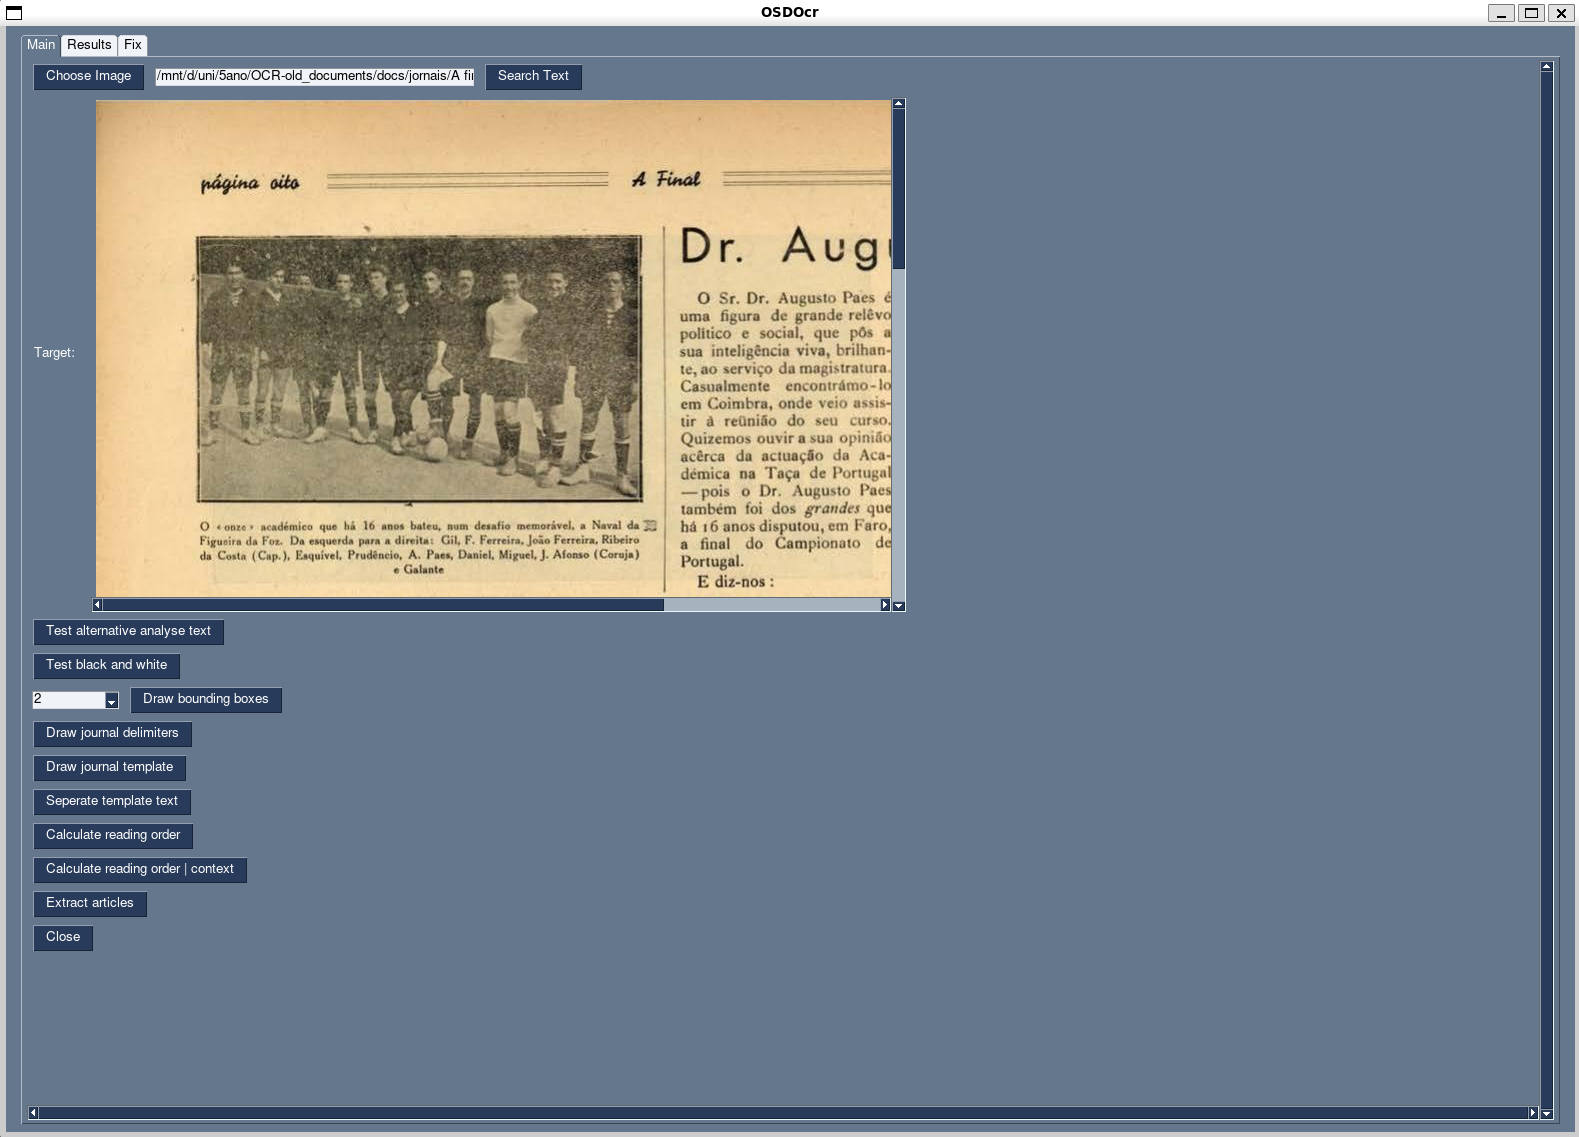
\includegraphics[width=1\textwidth]{images/implementacao/gui/gui_base.png}
%     \caption{Interface gráfica simples}
%     \label{fig:gui_base}
% \end{figure}
% 
% \subsubsection{Visualização de bounding boxes}
% 
% \begin{figure}[H]
%     \centering
%     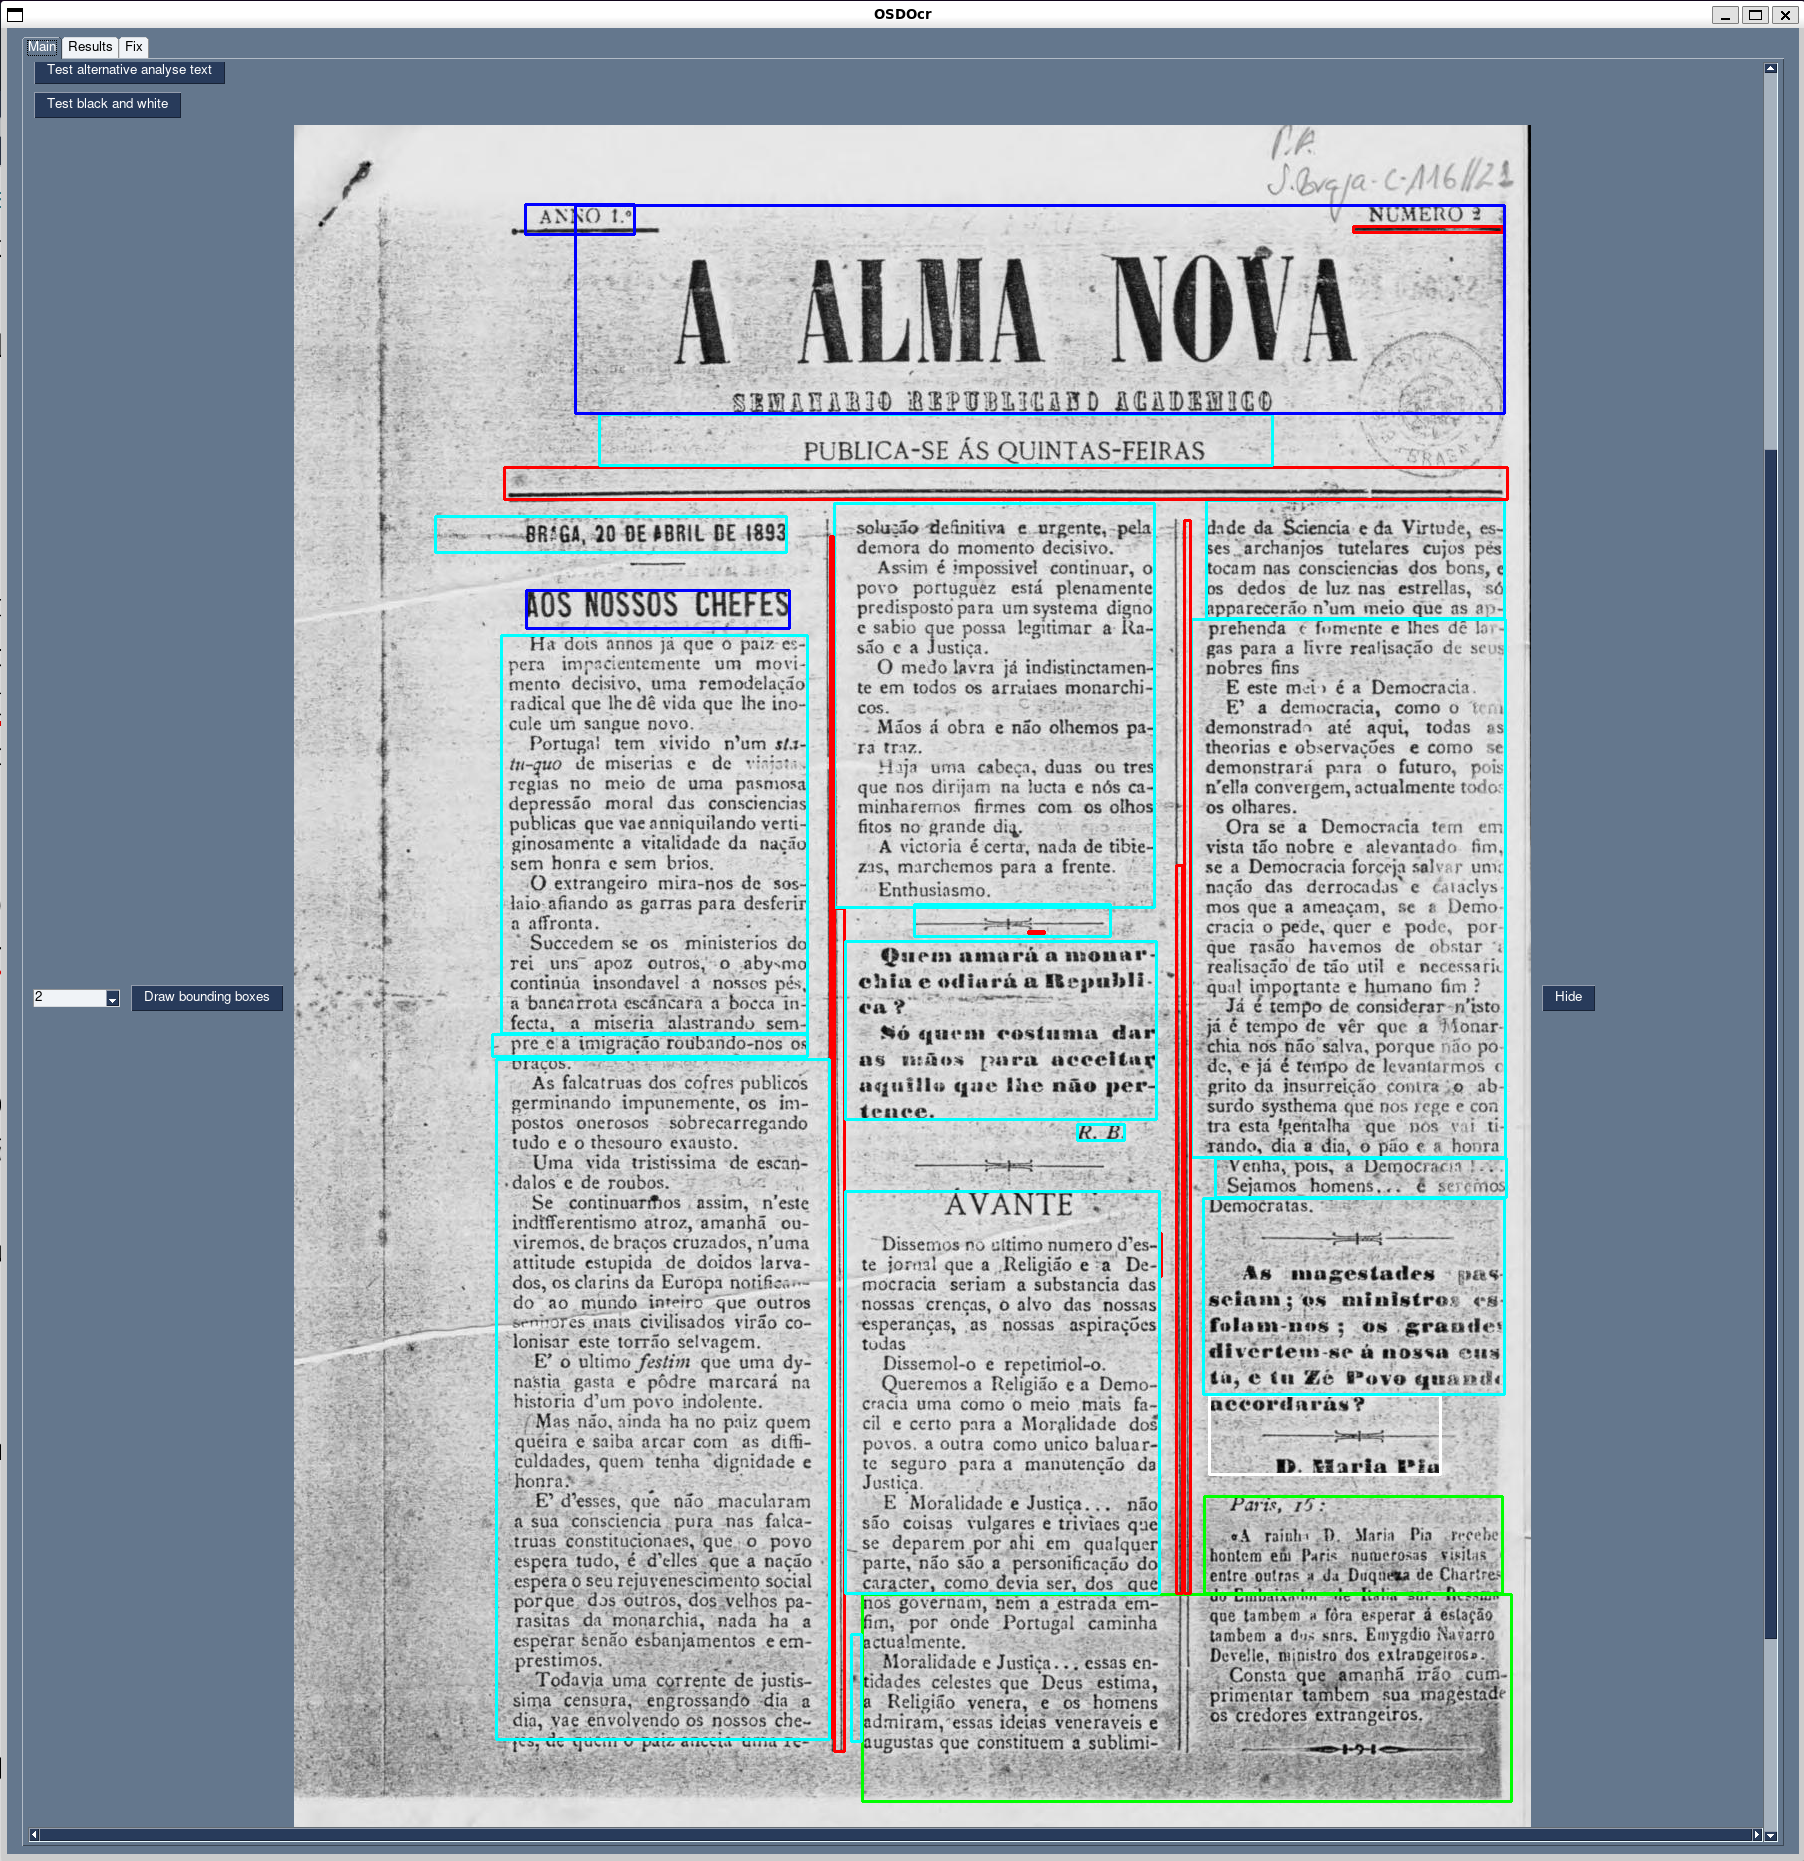
\includegraphics[width=1\textwidth]{images/implementacao/gui/gui_draw_bb.png}
%     \caption{Visualização dos blocos resultantes de OCR}
%     \label{fig:gui_draw_bb}
% \end{figure}
% 
% A visualização de blocos dispõe também de coloração diferente para os blocos de acordo com a sua categorização. Blocos título estão a azul escuro, texto a azul claro, delimitadores a vermelho, legendas a branco e o resto - imagens, outros - a verde.
% 
% \subsubsection{Cálculo de template de jornal}
% 
% \begin{figure}[H]
%     \centering
%     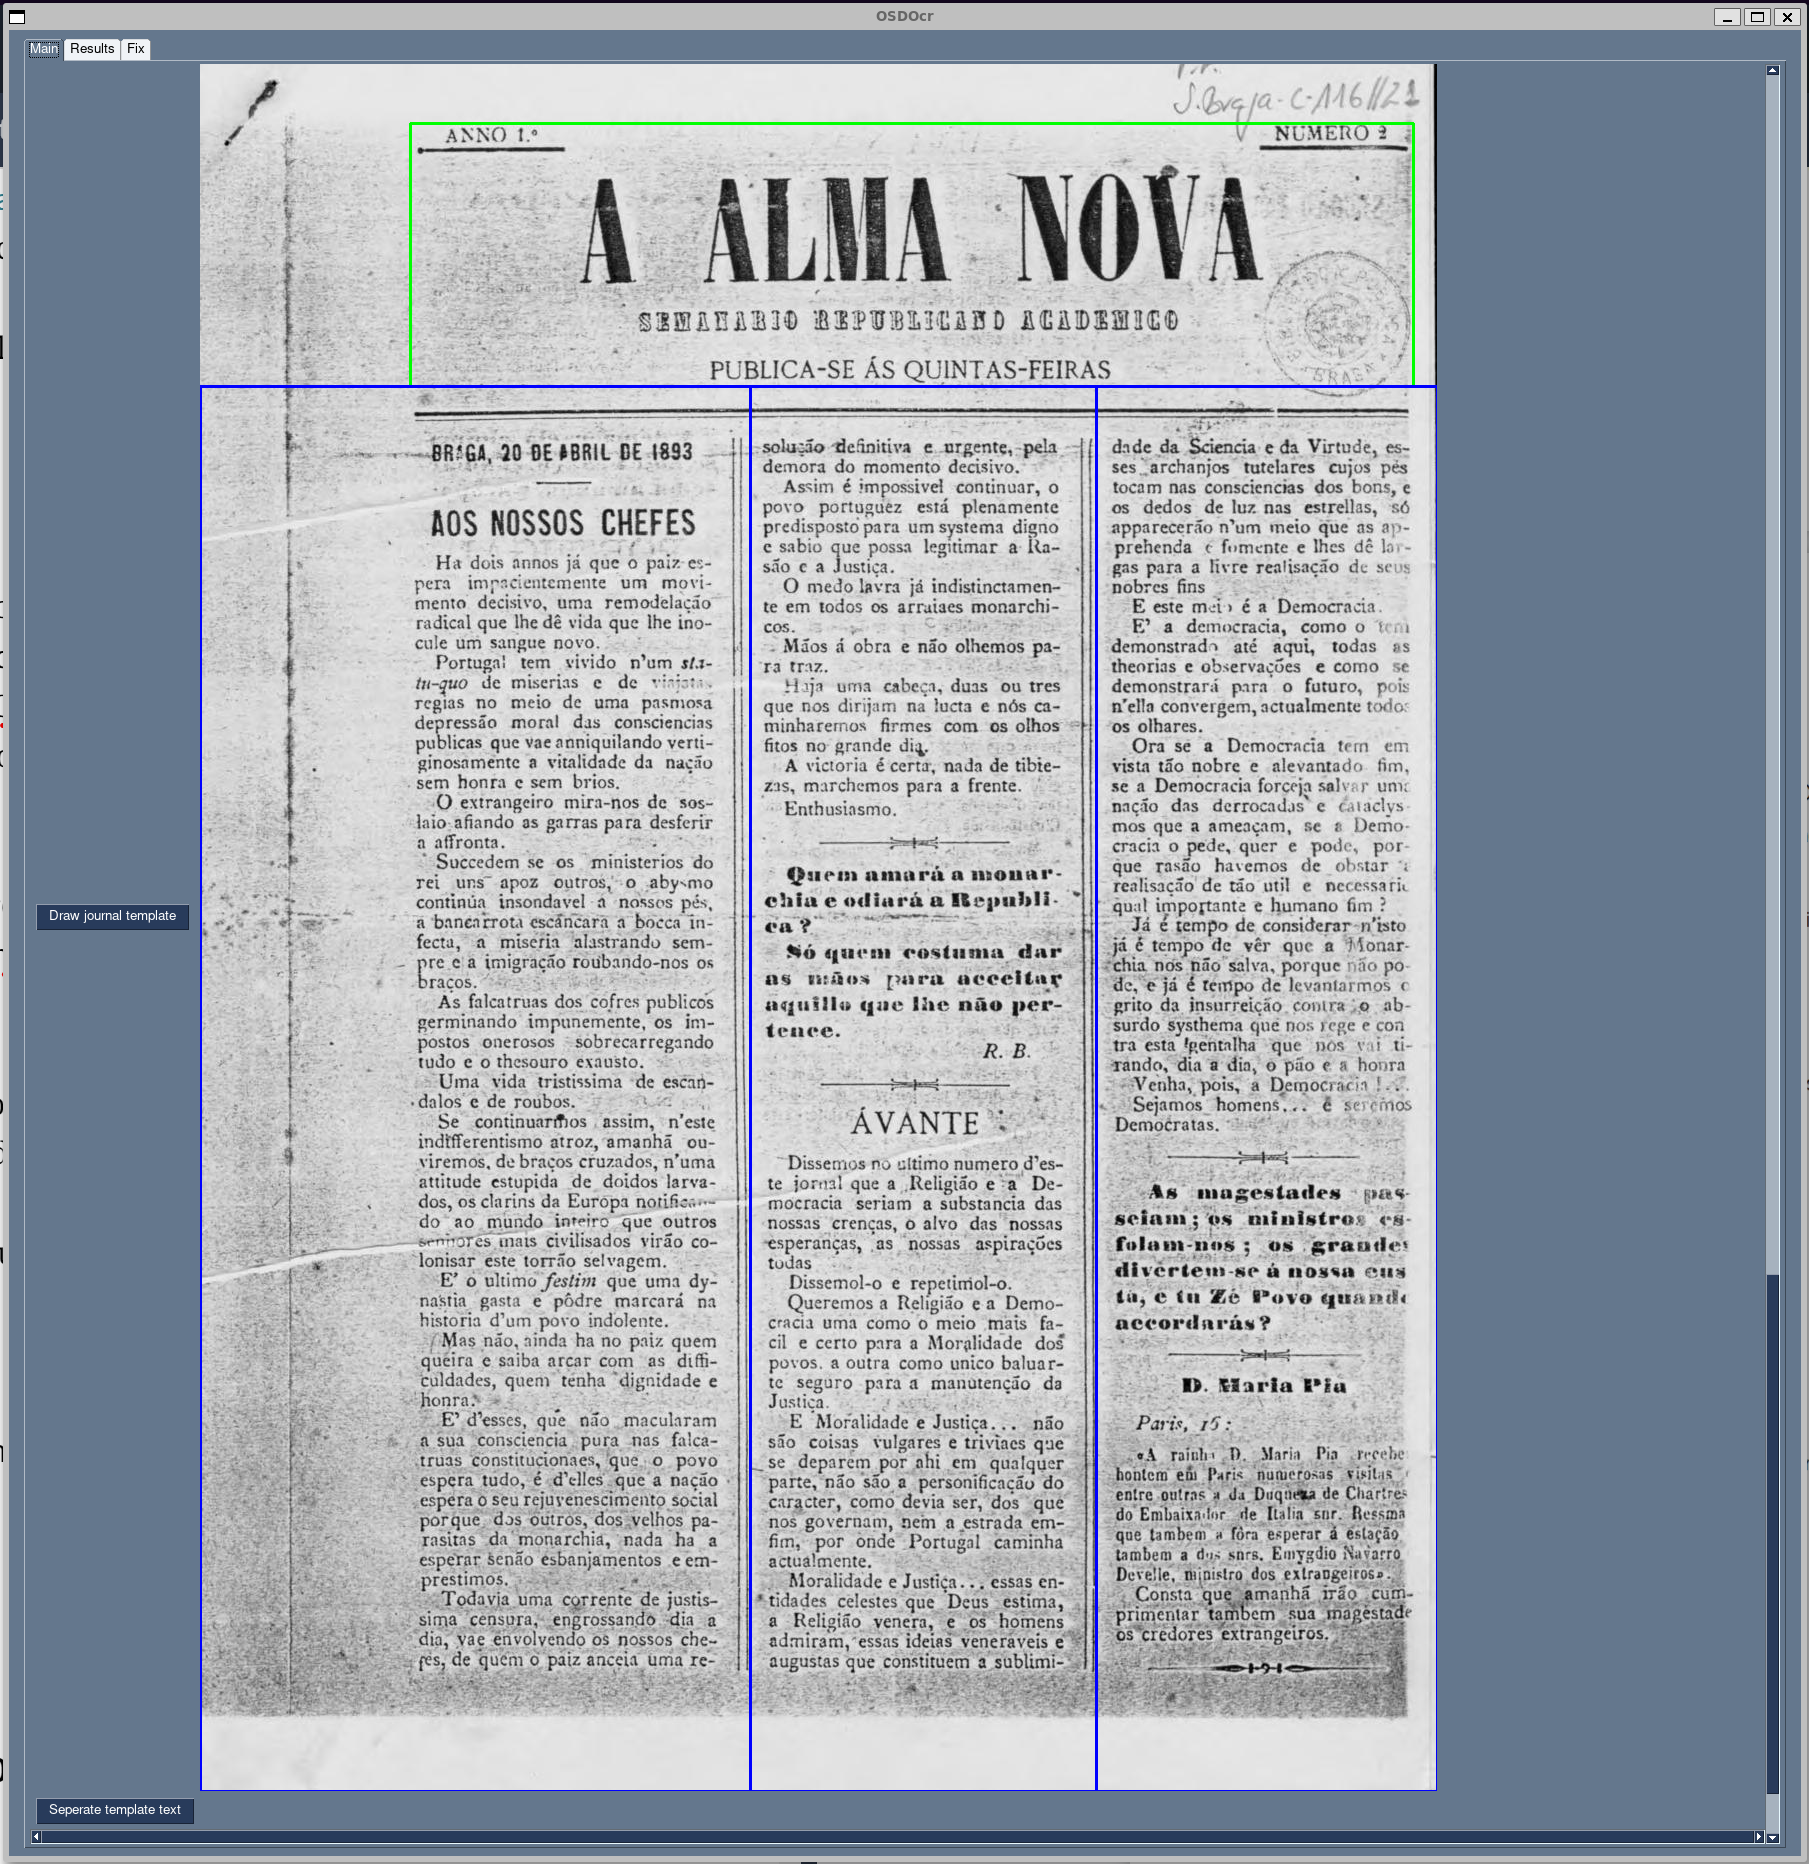
\includegraphics[width=1\textwidth]{images/implementacao/gui/gui_draw_template.png}
%     \caption{Visualização do cálculo do template de jornal}
%     \label{fig:gui_draw_template}
% \end{figure}
% 
% O cálculo de template é feito através da deteção e análise dos delimitadores dos resultados OCR. Áreas são depois calculadas de acordo com estes delimitadores e, como se pode ver no caso do Header (caixa a verde) da imagem \ref{fig:gui_draw_template}, a área é ajustada de acordo com as caixas com texto da respetiva área.
% 
% \subsubsection{Extração de artigos}
% 
% \begin{figure}[H]
%     \centering
%     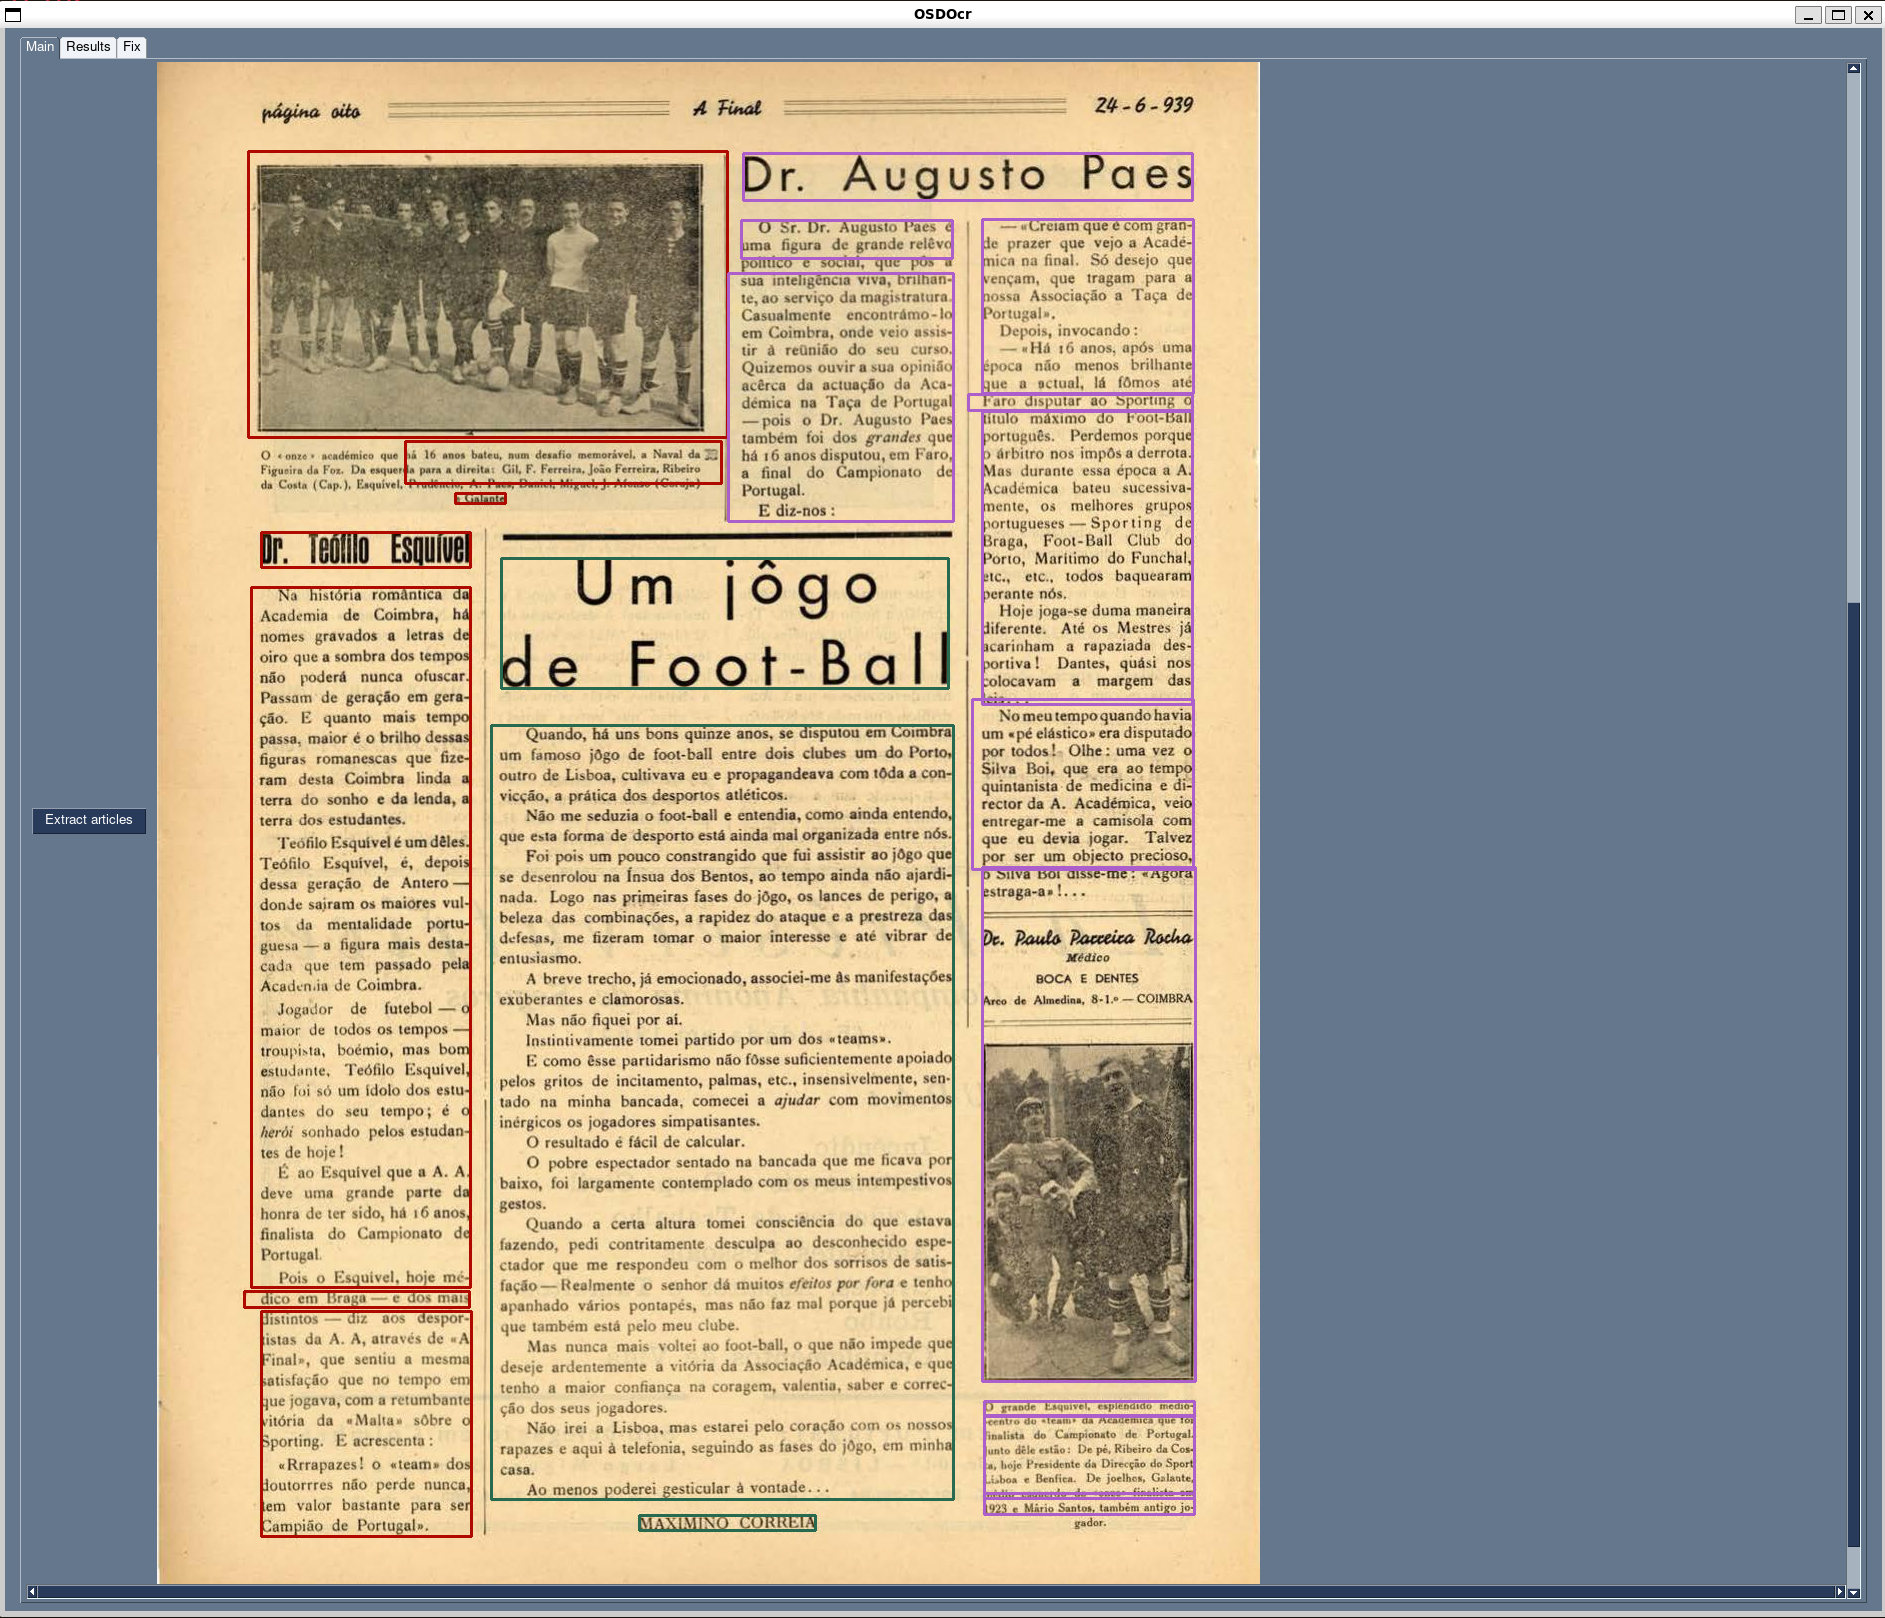
\includegraphics[width=1\textwidth]{images/implementacao/gui/gui_draw_articles.png}
%     \caption{Visualização dos artigos extraídos}
%     \label{fig:gui_draw_article}
% \end{figure}
% 
% Neste caso, os artigos são calculados e posteriormente escolhidas cores distintas para realçar cada um destes. Os artigos são representados pelo conjunto de blocos que foram agrupados como sendo um dado artigo.
% 
% \subsubsection{Limpeza de bounding boxes}
% 
% \begin{figure}[H]
%     \centering
%     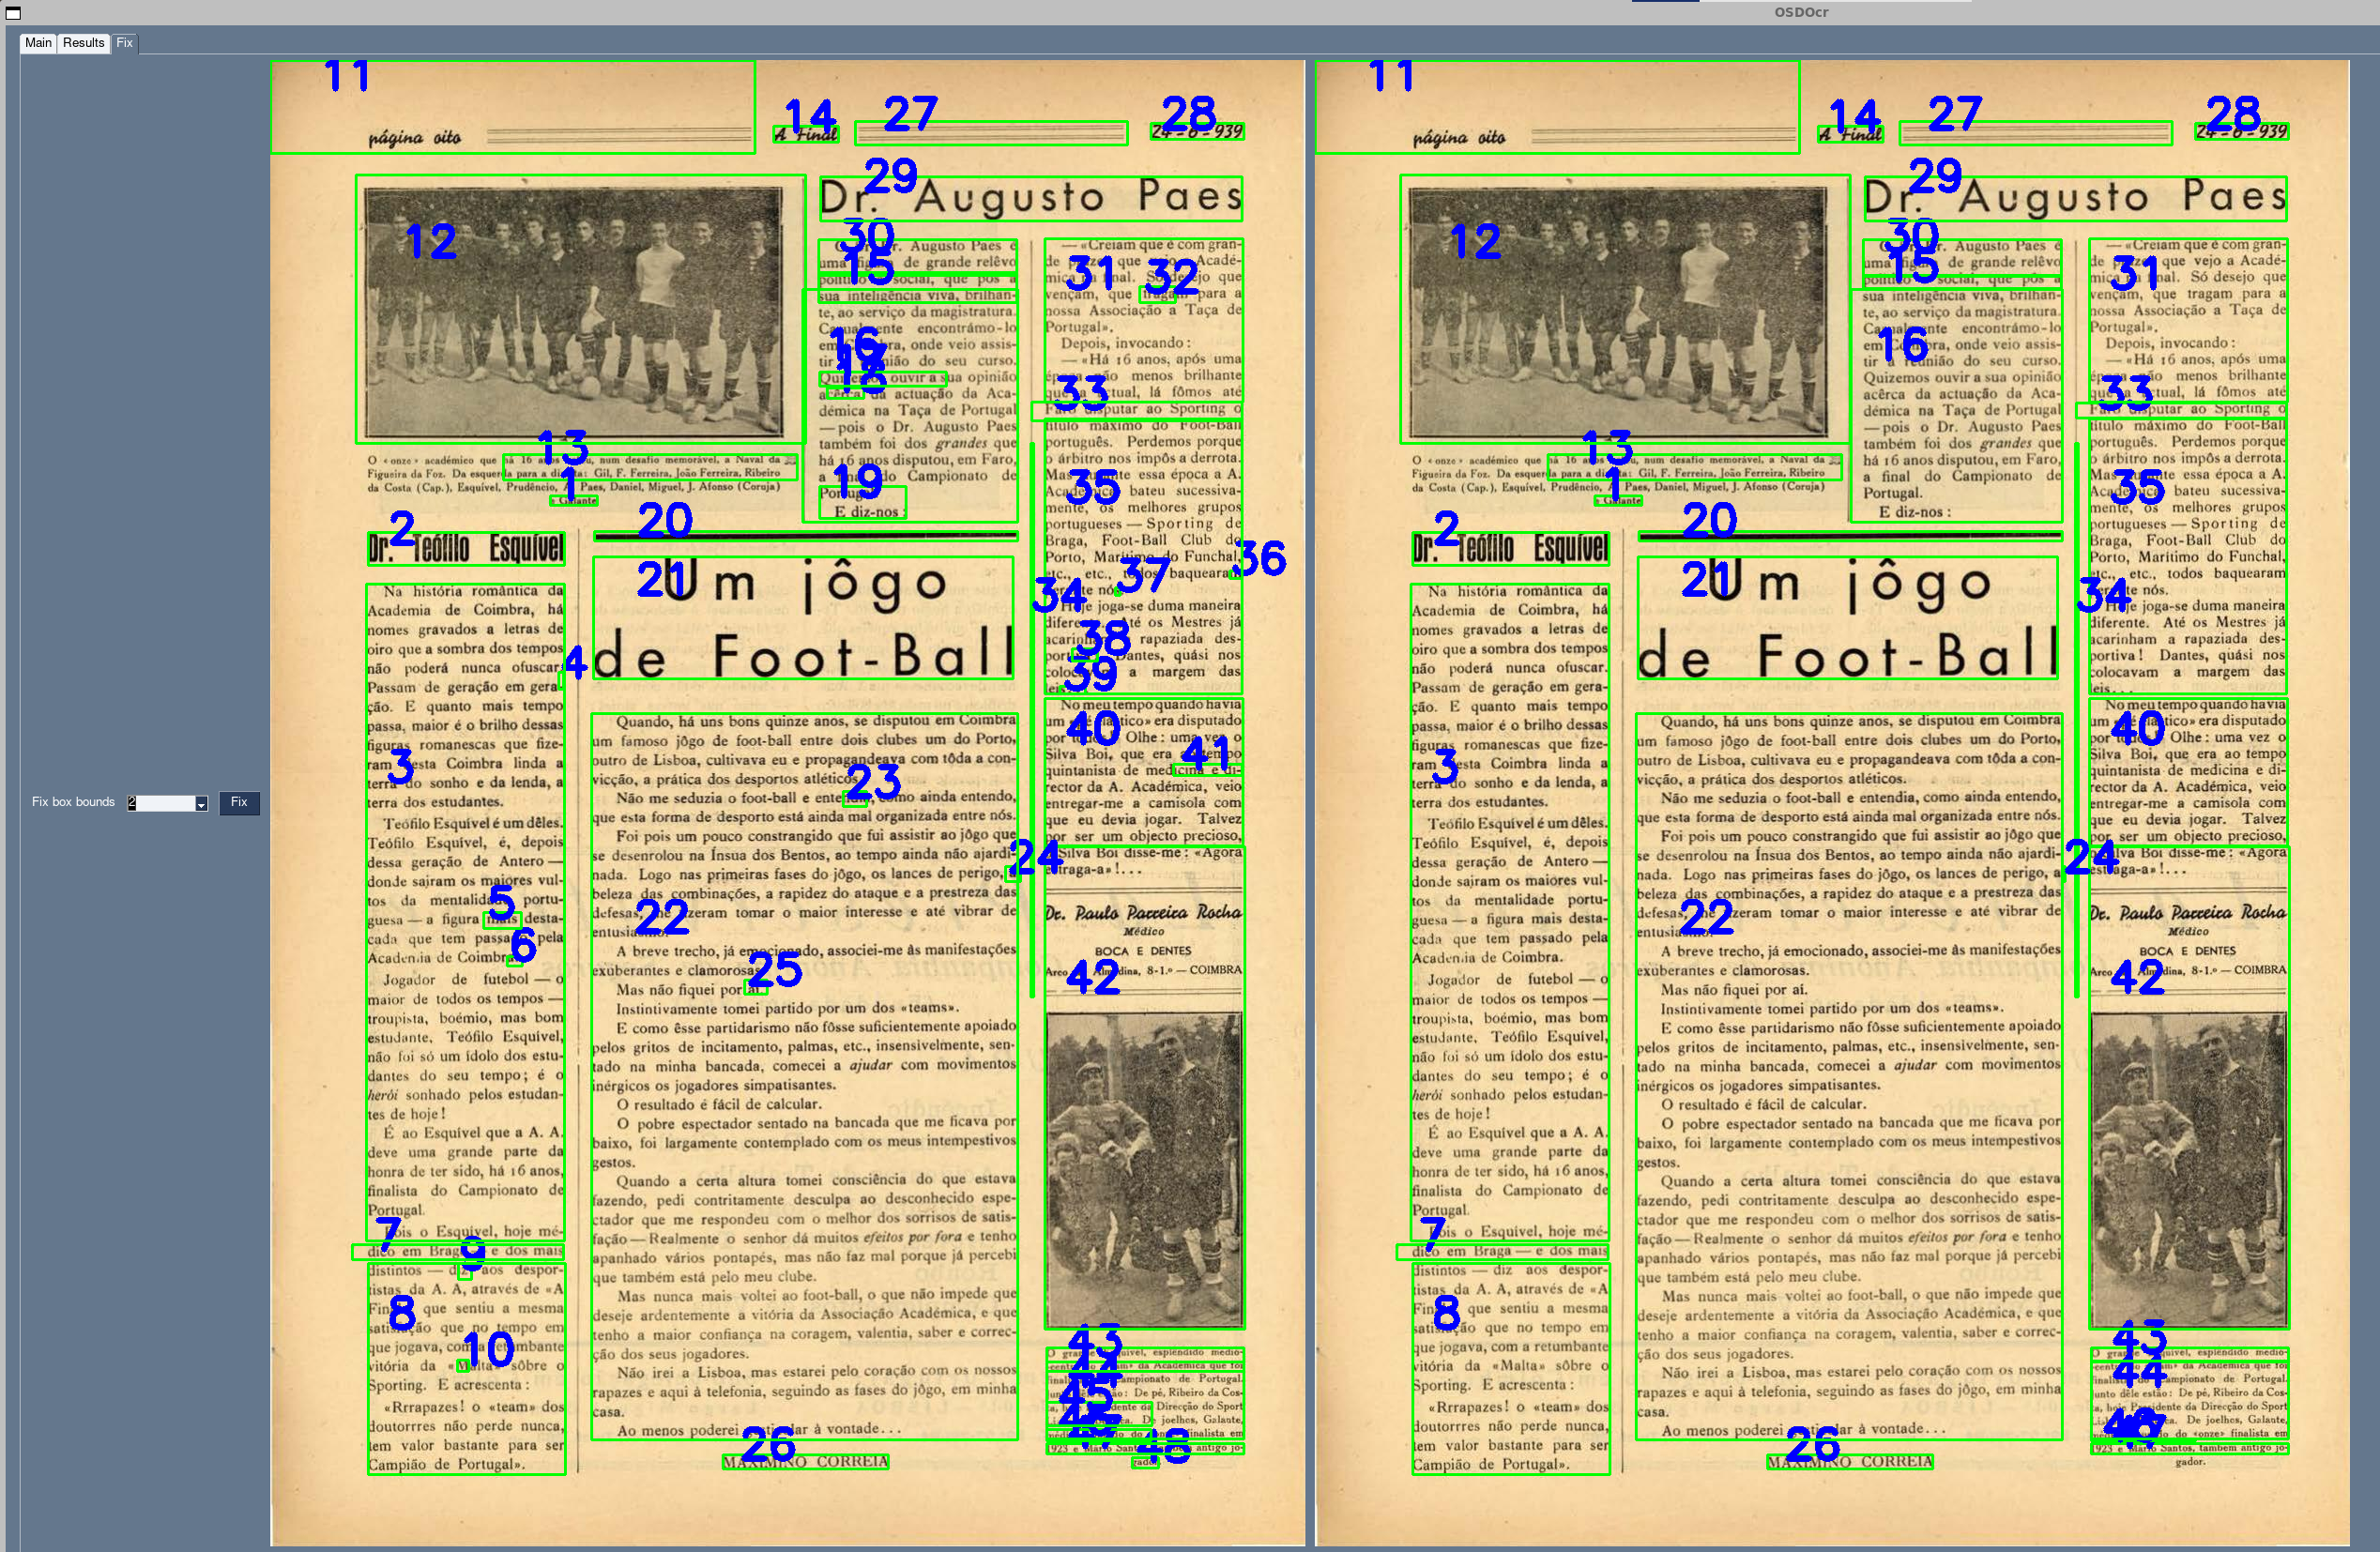
\includegraphics[width=1\textwidth]{images/implementacao/gui/gui_fix_blocks.png}
%     \caption{Visualização da limpeza de blocos}
%     \label{fig:gui_fix_bb}
% \end{figure}
% 
% Para facilitar a deteção das diferenças entre o antes e depois da limpeza, os dois estados são postos lado a lado e os blocos são identificados, mantendo a mesma identificação após a limpeza. 




